\documentclass[a4paper,11pt]{article}
\usepackage[a4paper,margin=1in,footskip=0.25in]{geometry}
\usepackage[utf8]{inputenc}


% science
\usepackage{amsmath}
\usepackage{array}
\usepackage{siunitx}

% code
% Default fixed font does not support bold face
\DeclareFixedFont{\ttb}{T1}{txtt}{bx}{n}{10} % for bold
\DeclareFixedFont{\ttm}{T1}{txtt}{m}{n}{10}  % for normal

% Custom colors
\usepackage{color}
\definecolor{deepblue}{rgb}{0,0,0.5}
\definecolor{deepred}{rgb}{0.6,0,0}
\definecolor{deepgreen}{rgb}{0,0.5,0}

\usepackage{listings}

% Python style for highlighting
\newcommand\pythonstyle{\lstset{
        language=Python,
        basicstyle=\ttm,
        morekeywords={self},              % Add keywords here
        keywordstyle=\ttb\color{deepblue},
        emph={MyClass,__init__},          % Custom highlighting
        emphstyle=\ttb\color{deepred},    % Custom highlighting style
        stringstyle=\color{deepgreen},
        frame=tb,                         % Any extra options here
        showstringspaces=false
}}

\newcommand\pythonstyleln{\lstset{
        language=Python,
        basicstyle=\ttm,
        morekeywords={self},              % Add keywords here
        keywordstyle=\ttb\color{deepblue},
        emph={MyClass,__init__},          % Custom highlighting
        emphstyle=\ttb\color{deepred},    % Custom highlighting style
        stringstyle=\color{deepgreen},
        frame=tb,                         % Any extra options here
        showstringspaces=false,
        numbers=left
}}

% Python environment
\lstnewenvironment{python}[1][]
{
    \pythonstyle
    \lstset{#1}
}
{}

\lstnewenvironment{pythonln}[1][]
{
    \pythonstyleln
    \lstset{#1}
}
{}

% Python for external files
\newcommand\pythonexternal[2][]{{
        \pythonstyle
        \lstinputlisting[#1]{#2}}}

% Python for inline
\newcommand\pythoninline[1]{{\pythonstyle\lstinline!#1!}}

% layout
\usepackage{float}
\usepackage{parskip}
\usepackage{graphicx}
\usepackage{longtable}
\usepackage{hyperref}
\usepackage[export]{adjustbox}
\usepackage{hhline}
\usepackage{chngcntr}

% referencing
\usepackage[style=apa]{biblatex}
\addbibresource{ratio.bib}

% table centering
\renewcommand{\arraystretch}{1.3}
\newcolumntype{P}[1]{>{\raggedright\arraybackslash}p{#1}}
\newcommand{\tptt}{$\times\,$}

% figures labelings
\usepackage{chngcntr}
\counterwithin{figure}{section}

\usepackage{caption}
\usepackage{subcaption}
\usepackage{wrapfig}

% fancy page numbers
\usepackage{fancyhdr}
% bottom right
\pagestyle{fancy}
\fancyhf{}
\fancyfoot[R]{\thepage}
\fancypagestyle{plain}{%
    \renewcommand{\headrulewidth}{0pt}%
    \fancyhf{}%
    \fancyfoot[R]{\thepage}%
}
%go
\renewcommand{\headrulewidth}{0pt}
\linespread{1.25}

% custom
\DeclareMathOperator{\di}{d\!}
\newcommand*\Eval[3]{\left.#1\right\rvert_{#3}^{#2}}


\usepackage{hyperref}

\title{\vspace{-8ex}Estimating the quality of YouTube videos based on its number of likes and dislikes}

\author{}
%\date{}
\date{\vspace{-8ex}}

\begin{document}

% Planning
% Introduction
% Definition
% Steps of exploration
% Simulation Approach
% Statistical Approach
% Bayensian Approach
% Conclusion



\maketitle

\section{Introduction}

\begin{wrapfigure}{r}{0.50\textwidth}
    \centering
    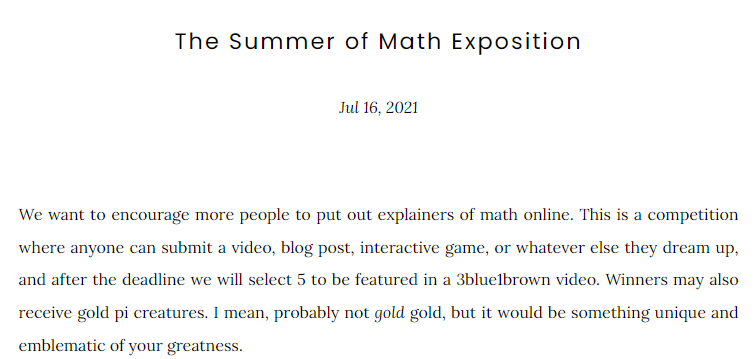
\includegraphics[width=0.48\textwidth]{assets/som1.png}
    \caption{The SoME1 event}
    \label{fig:some1}
\end{wrapfigure}

The topic of my exploration originates from a personal hobby I've developed in the school holidays.

Due to first year IB, I am familiar with the maths channel 3Blue1Brown (3B1B) on YouTube, for his videos are of high quality. When Grant (owner of 3B1B) announced a contest (figure \ref{fig:some1}) \parencite{sanderson} encouraging amateur video-makers to share their hidden maths knowledge, I was understandably very excited to have my entire YouTube home page filled with these new maths videos. While I did find some brilliantly made videos like ``The Beauty of B\'{e}zier Curves'' \parencite{holmer_2021}, and ``an explanation of Noether's Theorem'' \parencite{m_2021}, I quickly realized my inability to view all of the thousands of videos over a two week holiday. The solution? I will only watch the best ones.

But how do you tell if a YouTube video is the ``best'' out of the bunch? Visual indicators like interesting thumbnails is tempting, but I decided not to judge a book by its cover; while comparing view counts is fast, it is against the purpose of the maths event --- to discover new talented video creators. So I am left with the only other numerical indicators --- I want to judge the quality of the video through the number of likes and dislikes it has. While this measure can still contain subjectivity, it is certainly the most objective and interesting metric.

%(At the time of writing, the company YouTube has removed the dislike count on all videos, which is disappointing)

Therefore within this exploration, I will be finding an equation relating the number of likes and dislikes a YouTube video has to the best estimate of its perceived quality by the viewers. I will be using multiple methods such as simulations, statistical distributions, and a Bayesian approach to deduce the formula of video quality. I will evaluate the pros and cons of each approach, both in its results but also in its derivation. With the spirit of the contest, I chose to rank five random videos from the SoME1 event (table \ref{tbl:videos}).
%\begin{wrapfigure}{r}{0.4\textwidth}
%    \centering
%    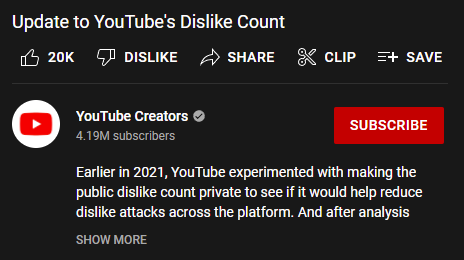
\includegraphics[width=0.45\textwidth]{assets/intro.png}
%    \caption{Hidden Dislikes}
%    \label{fig:hidden}
%\end{wrapfigure}

%This topic is chosen out of my curiously towards a very insignificant change. For I often procrastinate when doing my homework, I stumbled across a post on an online forum announcing the the popular internet video sharing platform of YouTube of removing their dislike counts (shown in Figure \ref{fig:hidden}). As usual, I dug into the comment section of the announcement and saw all the various complaints that one will expect on the internet, all but one has caught my eye:

%\begin{quote}
%    Dislike counts were necessary to spot clickbait, scams, fake tutorials, blatant misinformation, etc. --- Element 115 (internet user)
%\end{quote}

%The usage of likes and dislikes as a metric of legibility and quality is something that I knew and used extensively, mostly in saving my precious time in judging the qualities of the a series of maths videos made for the trend ``Summer of Math Exposition'' (SoME1) consisting of mostly amateur video makers. While the removal of the dislike counts demonstrated on how reliant I was on a simple number, it also led me to wonder of my technique in judging the quality of a video, especially in the SoME1 series for the like and dislike counts are often low. Therefore I felt this topic is worth exploring for its practicality.

% aim here

% 5 videos
% https://www.youtube.com/watch?v=-LVhZtFwZzM
% 705 2
% https://www.youtube.com/watch?v=E9IQY8LzzO8
% 35 5
% https://www.youtube.com/watch?v=vc_-aCeP7y8
% 25 0
% https://www.youtube.com/watch?v=tc53eCUvJyY
% 15 0 756
% https://www.youtube.com/watch?v=TJyCbR29Mds
% 4 0 138

\begin{figure}[H]
    \centering
    \begin{tabular}{c|c|c|c|c|c}
        & Video A & Video B & Video C & Video D & Video E \\
        \hline
        \hline
        Views & 138 & 440 & 467 & 756 & 10907 \\
        \hline
        Likes & 4 & 25 & 34 & 15 & 705 \\
        \hline
        Dislikes & 0 & 0 & 5 & 0 & 2
    \end{tabular}
    \captionof{table}{The statistics of the five videos at time of writing}
    \label{tbl:videos}
\end{figure}


\section{Ideas and Keywords}
First, we have to define some keywords that I used throughout the analysis. All YouTube videos are referred to as videos; the ratings of a video are its likes and dislikes, which are both positive integers; the likeability is the metric used to convey the quality of a video, and is represents a probability between 0 and 1, which can be defined as the mean probability of a viewer rating the video to select ``like''. (A likeability of $0.5$ means that a person rating the video is pressing the like button 50\% of the time) The focus would be to find a mathematical formula relating to this likeability.

Additionally, I am assuming that people can and will rate the video solely based on its quality --- the quality being the fundamental objective value. This eliminates rating from viewers who watched only a section of the video, or ratings given based on the creator and not the video it self. The assumption is both very idealistic and hard to confirm; notice that the five chosen videos have more views and ratings, revealing a potential bias towards the negative ratings for the satisfied viewers simply move on. This will restrict the scope of any models created in this essay, but I believe that the spirit of the contest --- to promote small creators --- will offset the usual biases, pushing these sample videos into the scope of the models.

\subsection{Naive likeability}
For my first attempt towards a formula of video likeabilities, consider video A and video C (table \ref{tbl:ex}).


\begin{figure}[H]
    \centering
    \begin{tabular}{c|c|c}
        & Video A & Video C \\
        \hline
        \hline
        Likes & 4 & 34\\
        \hline
        Dislikes & 0 & 6
    \end{tabular}
    \captionof{table}{}
    \label{tbl:ex}
\end{figure}

% the two videos
%\begin{figure}[H]
%    \centering
%    
\includegraphics[width=0.7\textwidth]{assets/s_vid2.png}
%    \caption{Video one \parencite{fluency_2021}}
%    \label{fig:vid1}
%\end{figure}

%\begin{figure}[H]
%    \centering
%    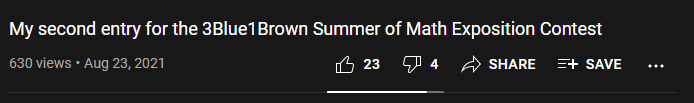
\includegraphics[width=0.7\textwidth]{assets/s_vid1.png}
%    \caption{Video two \parencite{division_2021}}
%    \label{fig:vid2}
%\end{figure}

Video A has 4 likes and 0 dislike. Video C has 34 likes and 6 dislikes. I found it tempting to define the likeability by the percentage of the likes received on a video, for I imagine likeability increases as the number of likes increase, and decreases as the number of dislikes increases. I will call this method the naive likeability, defined by:
\[
    L = \frac{x}{n},
\]
where $L$ is the naive likeability, $x$ is the amount of likes, and $n$ is the amount of ratings.

The naive likeabilities of video A ($L_1$) and video C ($L_2$) can thus be computed:
\begin{align*}
    L_{1} &= \frac{4}{4} = 1, \,\, L_{2} = \frac{34}{34 + 6} \approx 0.872
\end{align*}

If we assume this naive mathematical definition of the likeabilities represents my language definition, then the first video rates higher than the second because it has a higher likeability ($1 > 0.872$). So I should watch video A first, right?

Upon reflection, the calculations are unlikely to match my language definitions of likeability. Intuitively, it is very unlikely that 100\% of people will like video A because we saw just 4 likes --- the method failed to take the total amount of ratings into consideration. While video A has a higher like to dislike ratio than video C, there are fundamentally fewer overall ratings available.

This can be illustrated with an example taken to the extreme. A video with only one like and zero dislikes have a naive likeability of 100\%, but can we really be sure that it is of a higher quality than a video with 999 likes and 1 dislike (naive likeability of 99.9\%)?

\subsection{Naive Likeability Analysis}
Therefore the naive likeability definition is noninclusive of the rating amount, but is simple to compute even in ones head. I believe that it is a naive method to rate videos when the amount of ratings are small --- I hypothesis if the naive approach will be more accurate at higher amount of ratings, as most review sites utilize such ratios objectively. Nevertheless, table \ref{tbl:naive} shows the five videos as ranked by their naive likeabilities, showing that I should watch video A,B,D first, then video E and finally video C.

\begin{figure}[H]
    \centering
    \begin{tabular}{c|c|c|c|c|c}
        & Video A & Video B & Video C & Video D & Video E \\
        \hline
        \hline
        Naive Likeability (3dp) & 1.000 & 1.000 & 0.872 & 1.000 & 0.997
    \end{tabular}
    \captionof{table}{}
    \label{tbl:naive}
\end{figure}

Incidentally, the low amount of ratings assisted most sampled videos to a high naive likeability. Video A, B, and D all received a perfect likeability of 100\%, while naively indicating equal quality, it feels like that video B should be of higher quality than the others due to its larger ratings count of 25. Therefore I believe that a more inclusive approach would differentiate this perfect trio, ranking video B above the others.


\section{Simulation Approach}
For any statistical or probabilistic question, I always found it helpful to start with a simulation of some kind. This is because a simulation allows me to both describe the problem as well as to generate a numerical solution, guaranteed by the law of large numbers --- stating that the statistical descriptions of a sample will tend towards that of the true descriptions as sample size increases \parencite{dekking_kraaikamp_lopuhaä_meester_2005}.

% description of what I did
To do this, I've written a small piece of code that does the calculations in Python \parencite{python37}, and also used various Python libraries to make all the graphs that are used throughout this report \parencite{matplotlib} \parencite{numpy} \parencite{scipy}.

Using video A (4 likes and 0 dislike) as an example, I thought to define the likeability of a video by the average of all the possible likeabilities weighted by how likely they are to occur, as it matches my literal definition of ``the mean probability of a viewer rating the video to select like''.

\subsection{Simulation Method}
The pseudocode for our simulation is
\begin{python}
1   weighted = 0
2   for likeability in 0..1:
3       occurrence = simulate_occurrence(likeability)
4
5       weighted += likeability * occurrence / sample_size
6       plot(likeability, occurrence)
\end{python}

I will attempt to breakdown this piece of code line by line. Firstly, I defined a variable \pythoninline{weighted} to hold the weighted average of the likeabilties:
\begin{python}
1   weighted = 0
\end{python}

Then I loop over all possible likeabilities from 0 to 1 using a \textit{for in} loop:
\begin{python}
2   for likeability in 0..1:
\end{python}

For each likability, I considered a simulation of 1000 times a group of 4 people rating the video. This is performed by the function \pythoninline{simulate_occurrence}(full source code in appendix \ref{apd:sim_occ}), which takes the likeability as an input. It outputs the number of times the ratings by those 4 people matches the 4 likes and 0 dislike of video A and saves this in the variable called \pythoninline{occurrence}.
\begin{python}
3       occurrence = simulate_occurrence(likability)
\end{python}

To calculate the weighted averages (statistical mean) of the likeability, I've used the discrete mean formula, which states the mean ($\mu$) is the sum of the likeabilities ($L_i$) multiplied by their respective probabilities ($f(L_i)$):
\[
    \mu = \sum_{i = 1}^{n} L_i f(L_i)
\]

The probabilities of each possible likeability is total occurrence divided by the \pythoninline{sample_size} of 1000. The summation is reflected by adding each weighted likeability to the \pythoninline{weighted} variable for each possible likeability:
\begin{python}
5       weighted += likeability * occurrence / sample_size
\end{python}

Finally, I decided to plot the relationship between \pythoninline{occurrence} against \pythoninline{likeability}. This is done by the \pythoninline{plot} function imported from Matplotlib:
\begin{python}
6       plot(likeability, occurrence)
\end{python}

% optional
%\newpage


To see the output, I ran the program with the parameters of 4 likes and 0 dislike from video one, and 1000 samples later I was greeted with the graph in figure \ref{fig:sim_ratings_v1}.

\begin{figure}[H]
    \centering
    \begin{minipage}{.5\textwidth}
        \centering
        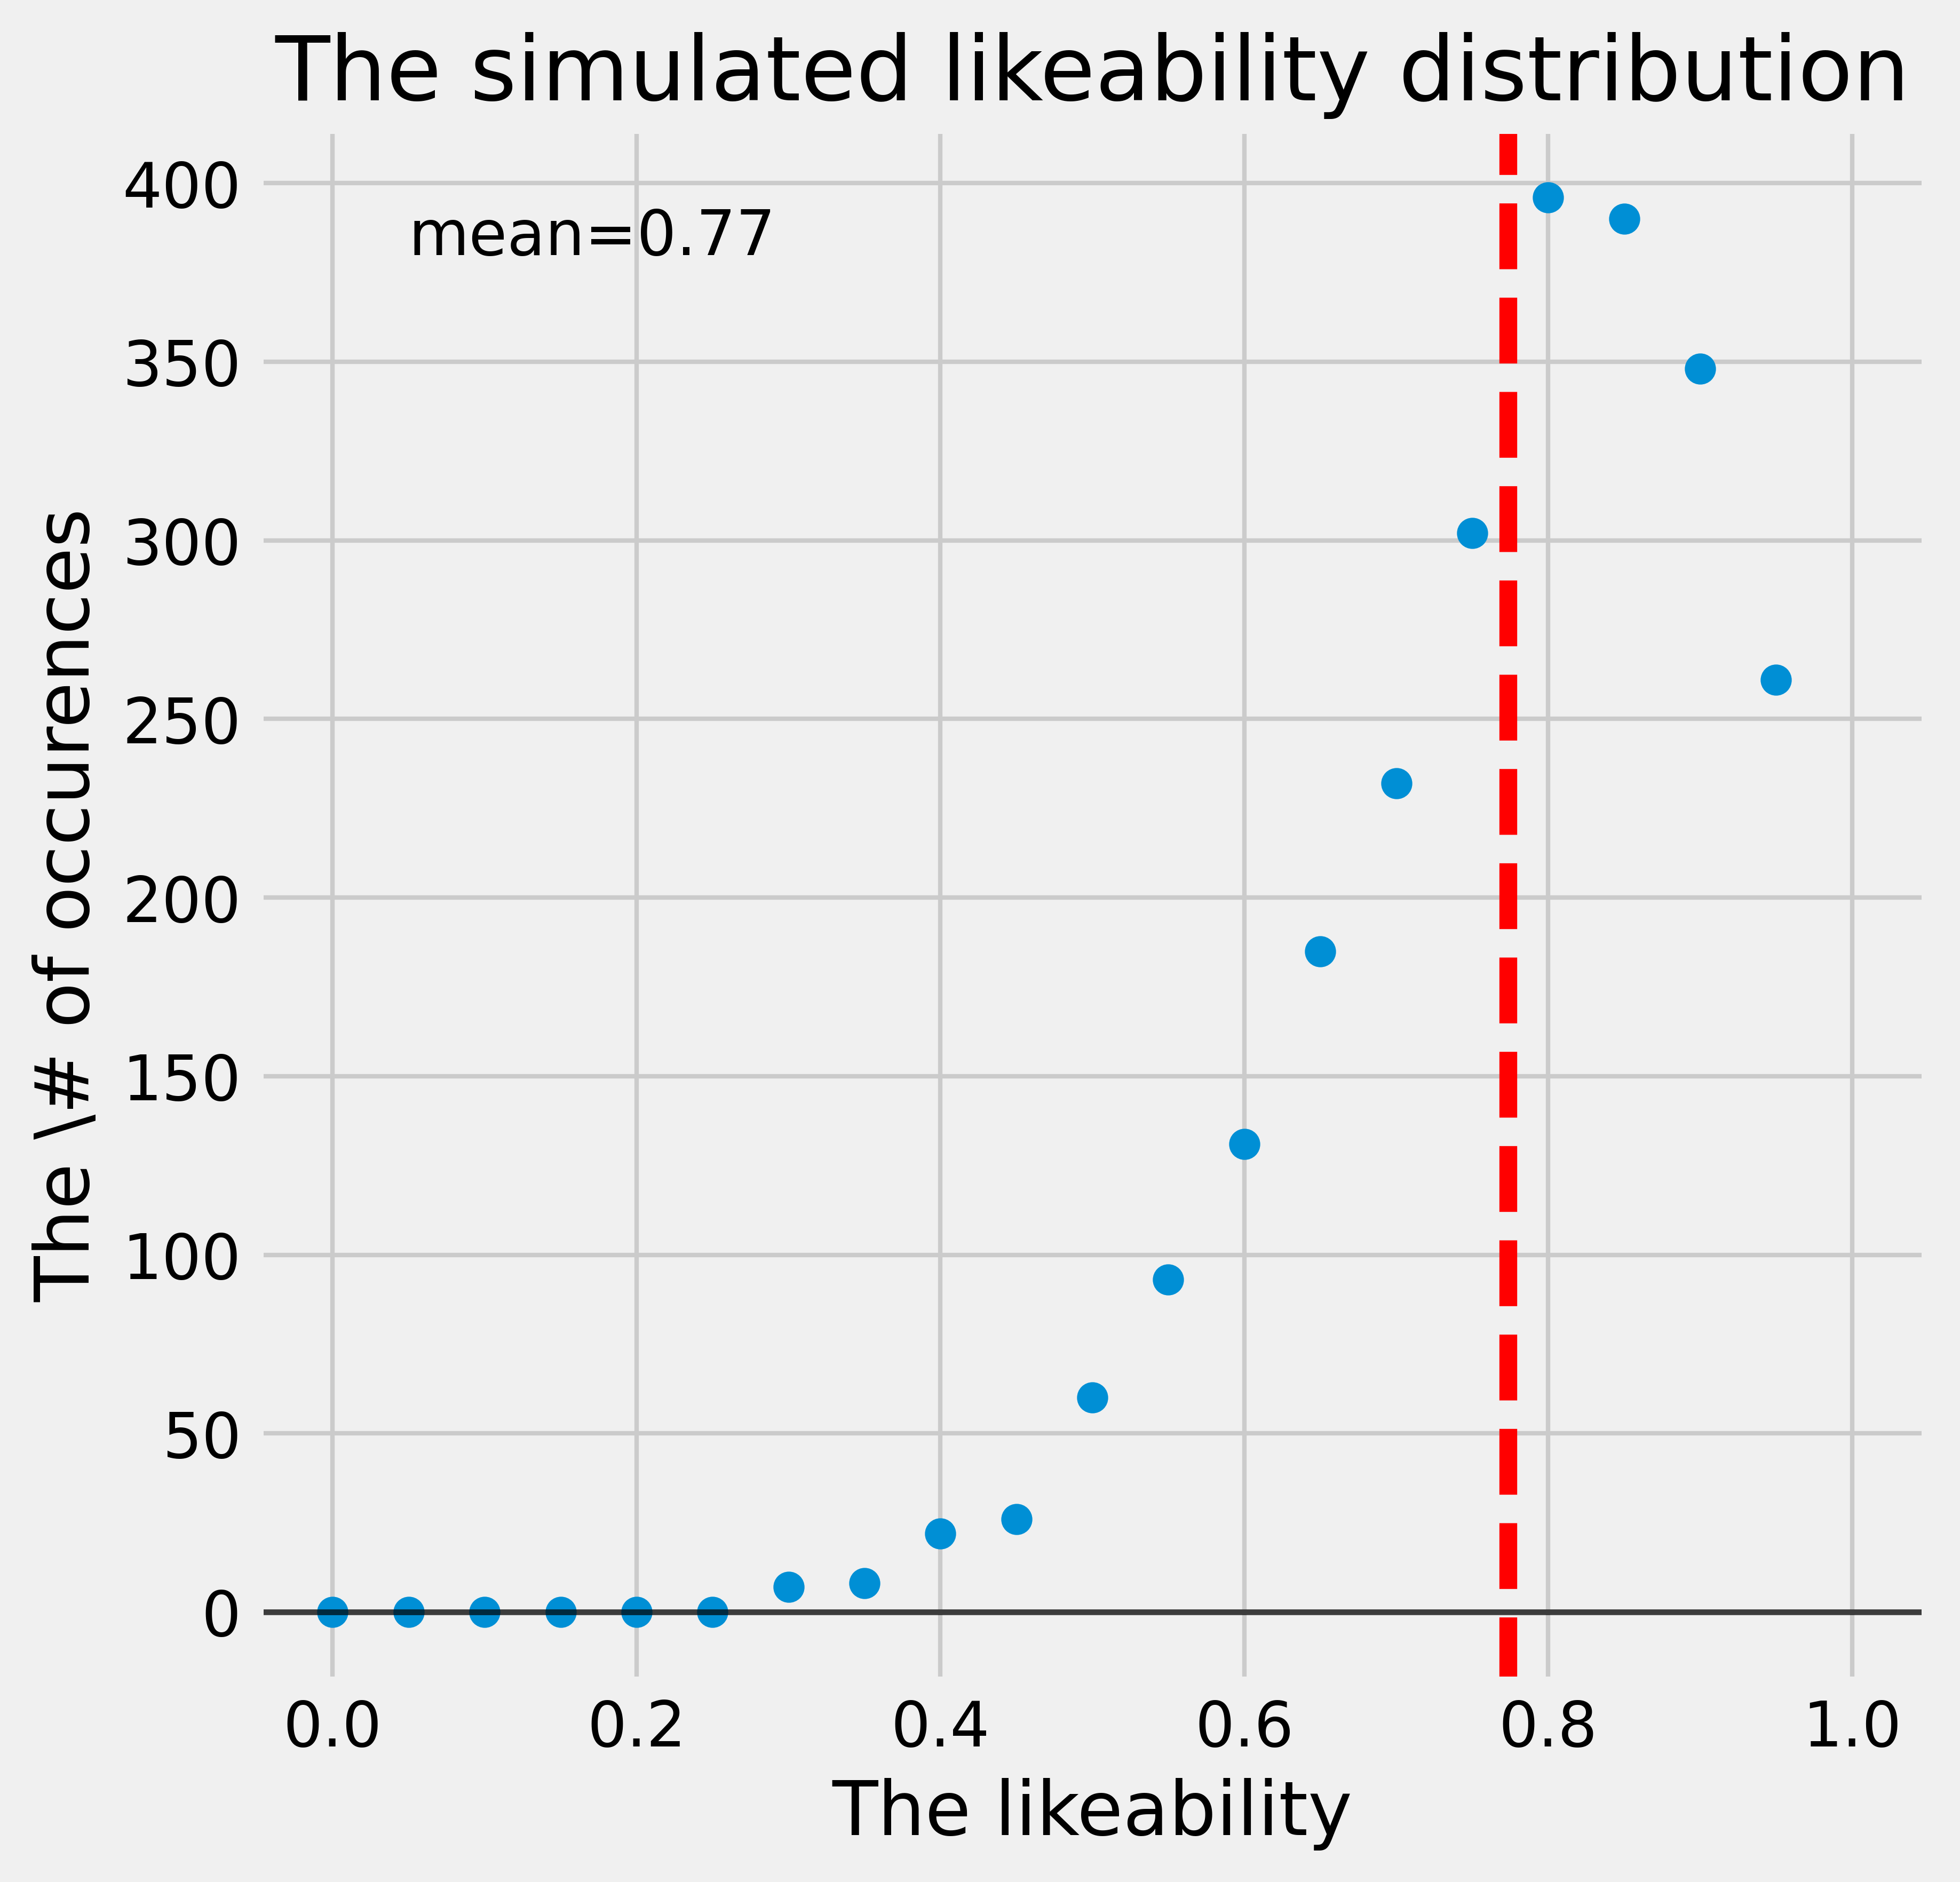
\includegraphics[width=0.9\linewidth]{assets/sim_ratings_v1.png}
        \caption{For video A}
        \label{fig:sim_ratings_v1}
    \end{minipage}%
    \begin{minipage}{.5\textwidth}
        \centering
        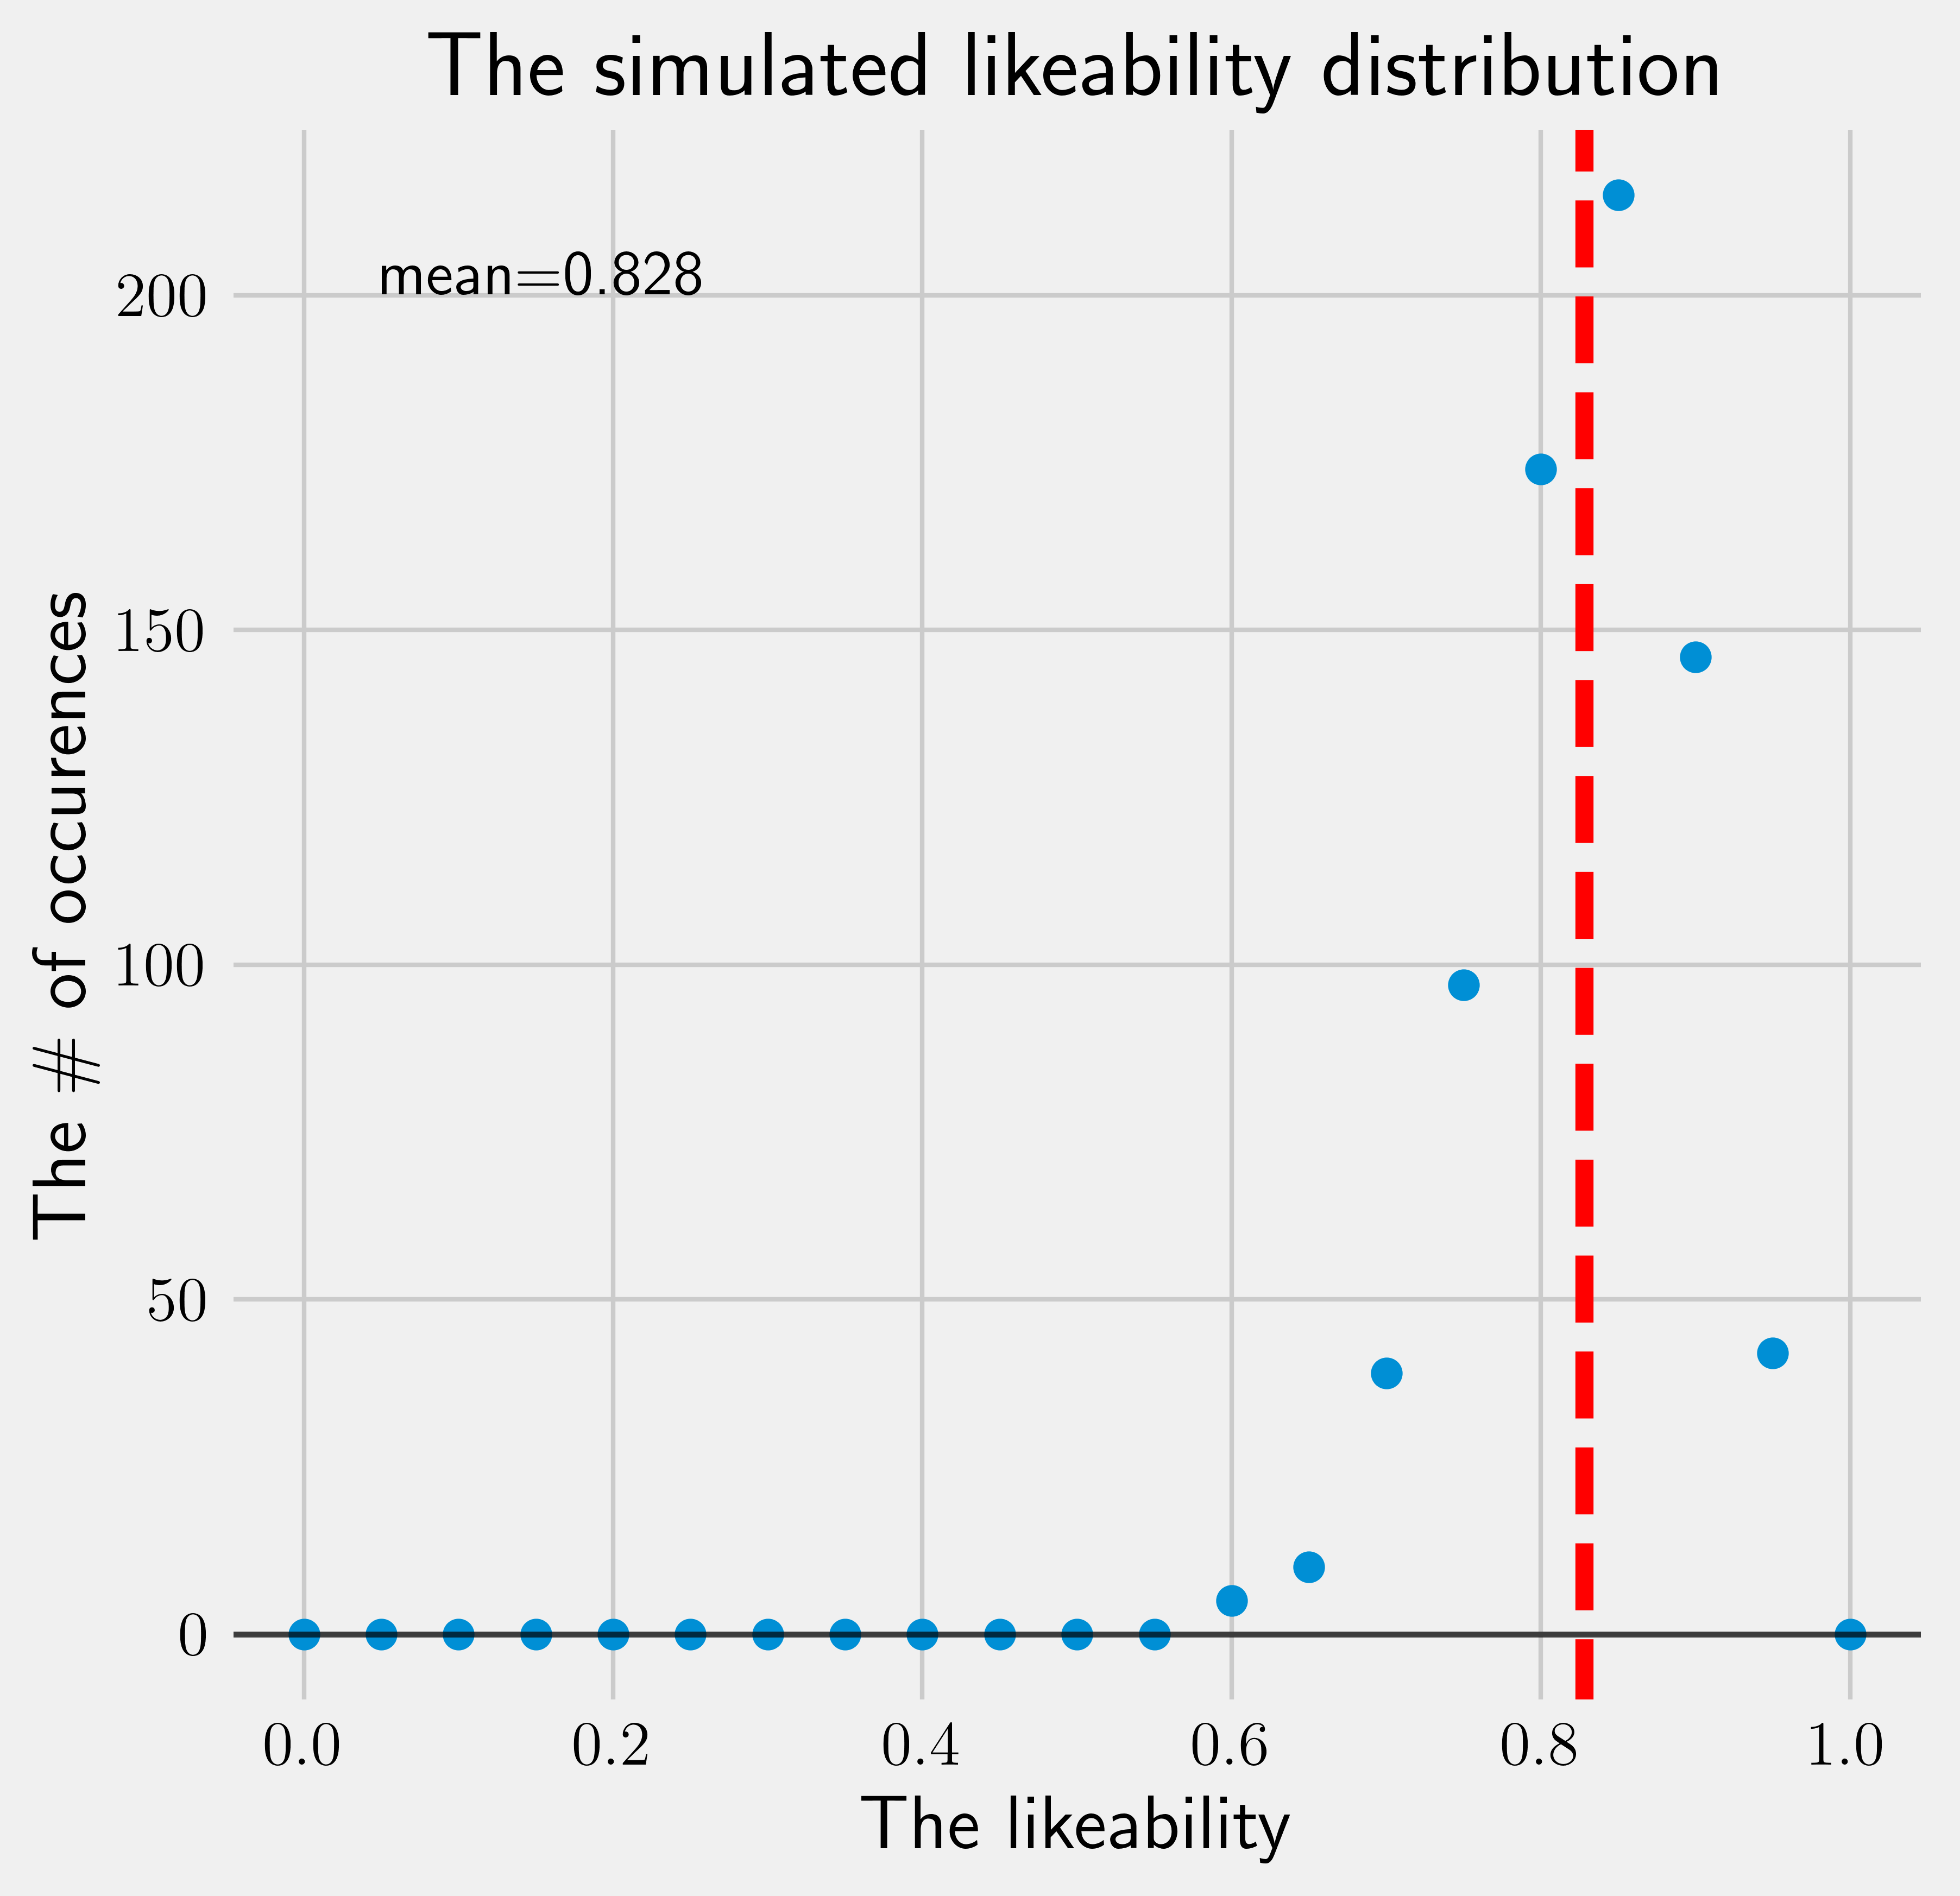
\includegraphics[width=0.9\linewidth]{assets/sim_ratings_v2.png}
        \caption{For video C}
        \label{fig:sim_ratings_v2}
    \end{minipage}
\end{figure}

\subsection{Simulation Analysis}
The blue dots in figure \ref{fig:sim_ratings_v1} represents the simulated occurrence of the video ratings out of 1000 samples of a chosen likeability (the likeabilities are selected with steps of 0.01 for clarity). The red vertical line graphs the mean likeability.

The graph was both an expected and unexpected turnout. The simulation placed the likeability of video at $0.838$, this is expected for there is certainly very little information available in only 4 ratings, but unexpected in size of the difference ($1-0.838=0.162$) against the naive likeability. This confirms my suspicion that the naive likeability overvalued the true likeability of the video for.

By running the program with the parameters of the second video with 34 likes and 6 dislikes,
I've obtained a mean of $0.857$ and figure \ref{fig:sim_ratings_v2}.

In comparison with its naive likeability, video C is less affected by the lack of information for the simulated likeability has a much smaller difference ($0.872-0.857=0.015$) than that of video one's. This partially confirmed my hypothesis of the naive method gaining accuracy at larger rating counts (tested in appendix \ref{apd:acc}), and could justify the use of the naive likeability to judge popular videos.

The shape of the graphs are also worth noting.
While the two figures are very distinct in shape and symmetry, I've noticed that the peak x-value of the graphs are the naive likeabilities of the videos. This is in contrast to the statistical mean of the graphs, which leans closer to the middle and away from the peak. Statistically, this is a comparison between mode and means, and the skewness of the distributions seemed to affect the exact differences between the mode and the mean. I wonder if when the graphs are symmetrical (like a normal distribution), the naive likeability really does equate to the correct likeability.

%They very much resemble a hill shaped curve that has a peek at only one likeability, and slopes increasing shallower the further away from the peek. Interestingly, the chosen metric of the statistical mean does not reflect the peek of the curve --- the red line does not intersect at the top of the curve. I believe this has to do with the long tail of zero occurrences at lower likeabilities, for they decrease the statistical mean in calculations.

% conclusion
Nevertheless, the simulation approach had proved to be helpful in framing the question in finding the so-called statistical mean of the range of possible likeabilities. On top of that, it had created a numerical method of estimating the likeability of videos. But it does come at a cost of precision and computational time, making the method unreliable and expensive to scale up to higher amounts of ratings. Table \ref{tbl:simulation} lists the five videos and their simulated likeability values with a sample size of 1000, and step 0.01.

\begin{figure}[H]
    \centering
    \begin{tabular}{c|c|c|c|c|c}
        & Video A & Video B & Video C & Video D & Video E \\
        \hline
        \hline
        Simulated Likeability (3dp) & 0.828 & 0.958 &  0.853 & 0.937 & 0.987
    \end{tabular}
    \captionof{table}{}
    \label{tbl:simulation}
\end{figure}

Two things are to be highlighted here. Firstly notice the slight variations in the simulated likeability values of video A,C, which I believe is caused by the random number generators. While larger sample sizes could reduce the variations at the cost of computational time, such errors may reduce the validity of the results during comparisons. Secondly notice that this metric of likeability had video C exceed video A, opposite of the conclusions made in the naive likeability section. It also confirmed my hypothesis that video B will score higher than video A,D --- this likeability measurement seems to be what I am looking for.

\section{Statistical Approach}

% what are distributions
To formalize and reduce the variations of the simulation approach, I sought for a analytic equation of the likeability metric. Remember that the simulation was used to compute the occurrences of a given rating for all ranges of likeabilities, and the statistical mean of the curve it creates is the simulated likeability of the video. It may be helpful to define this curve more mathematically without the element of chance in the occurrence function.

% examples of distributions
\subsection{Continuous Random Variables and Prior Distribution}
Firstly, the likeability of a video can be thought of as a continuous random variable of symbol $L$ of domain $[0, 1]$, as the likeability can range from 0\% to 100\%.
%\begin{wrapfigure}{r}{0.45\textwidth}
 %   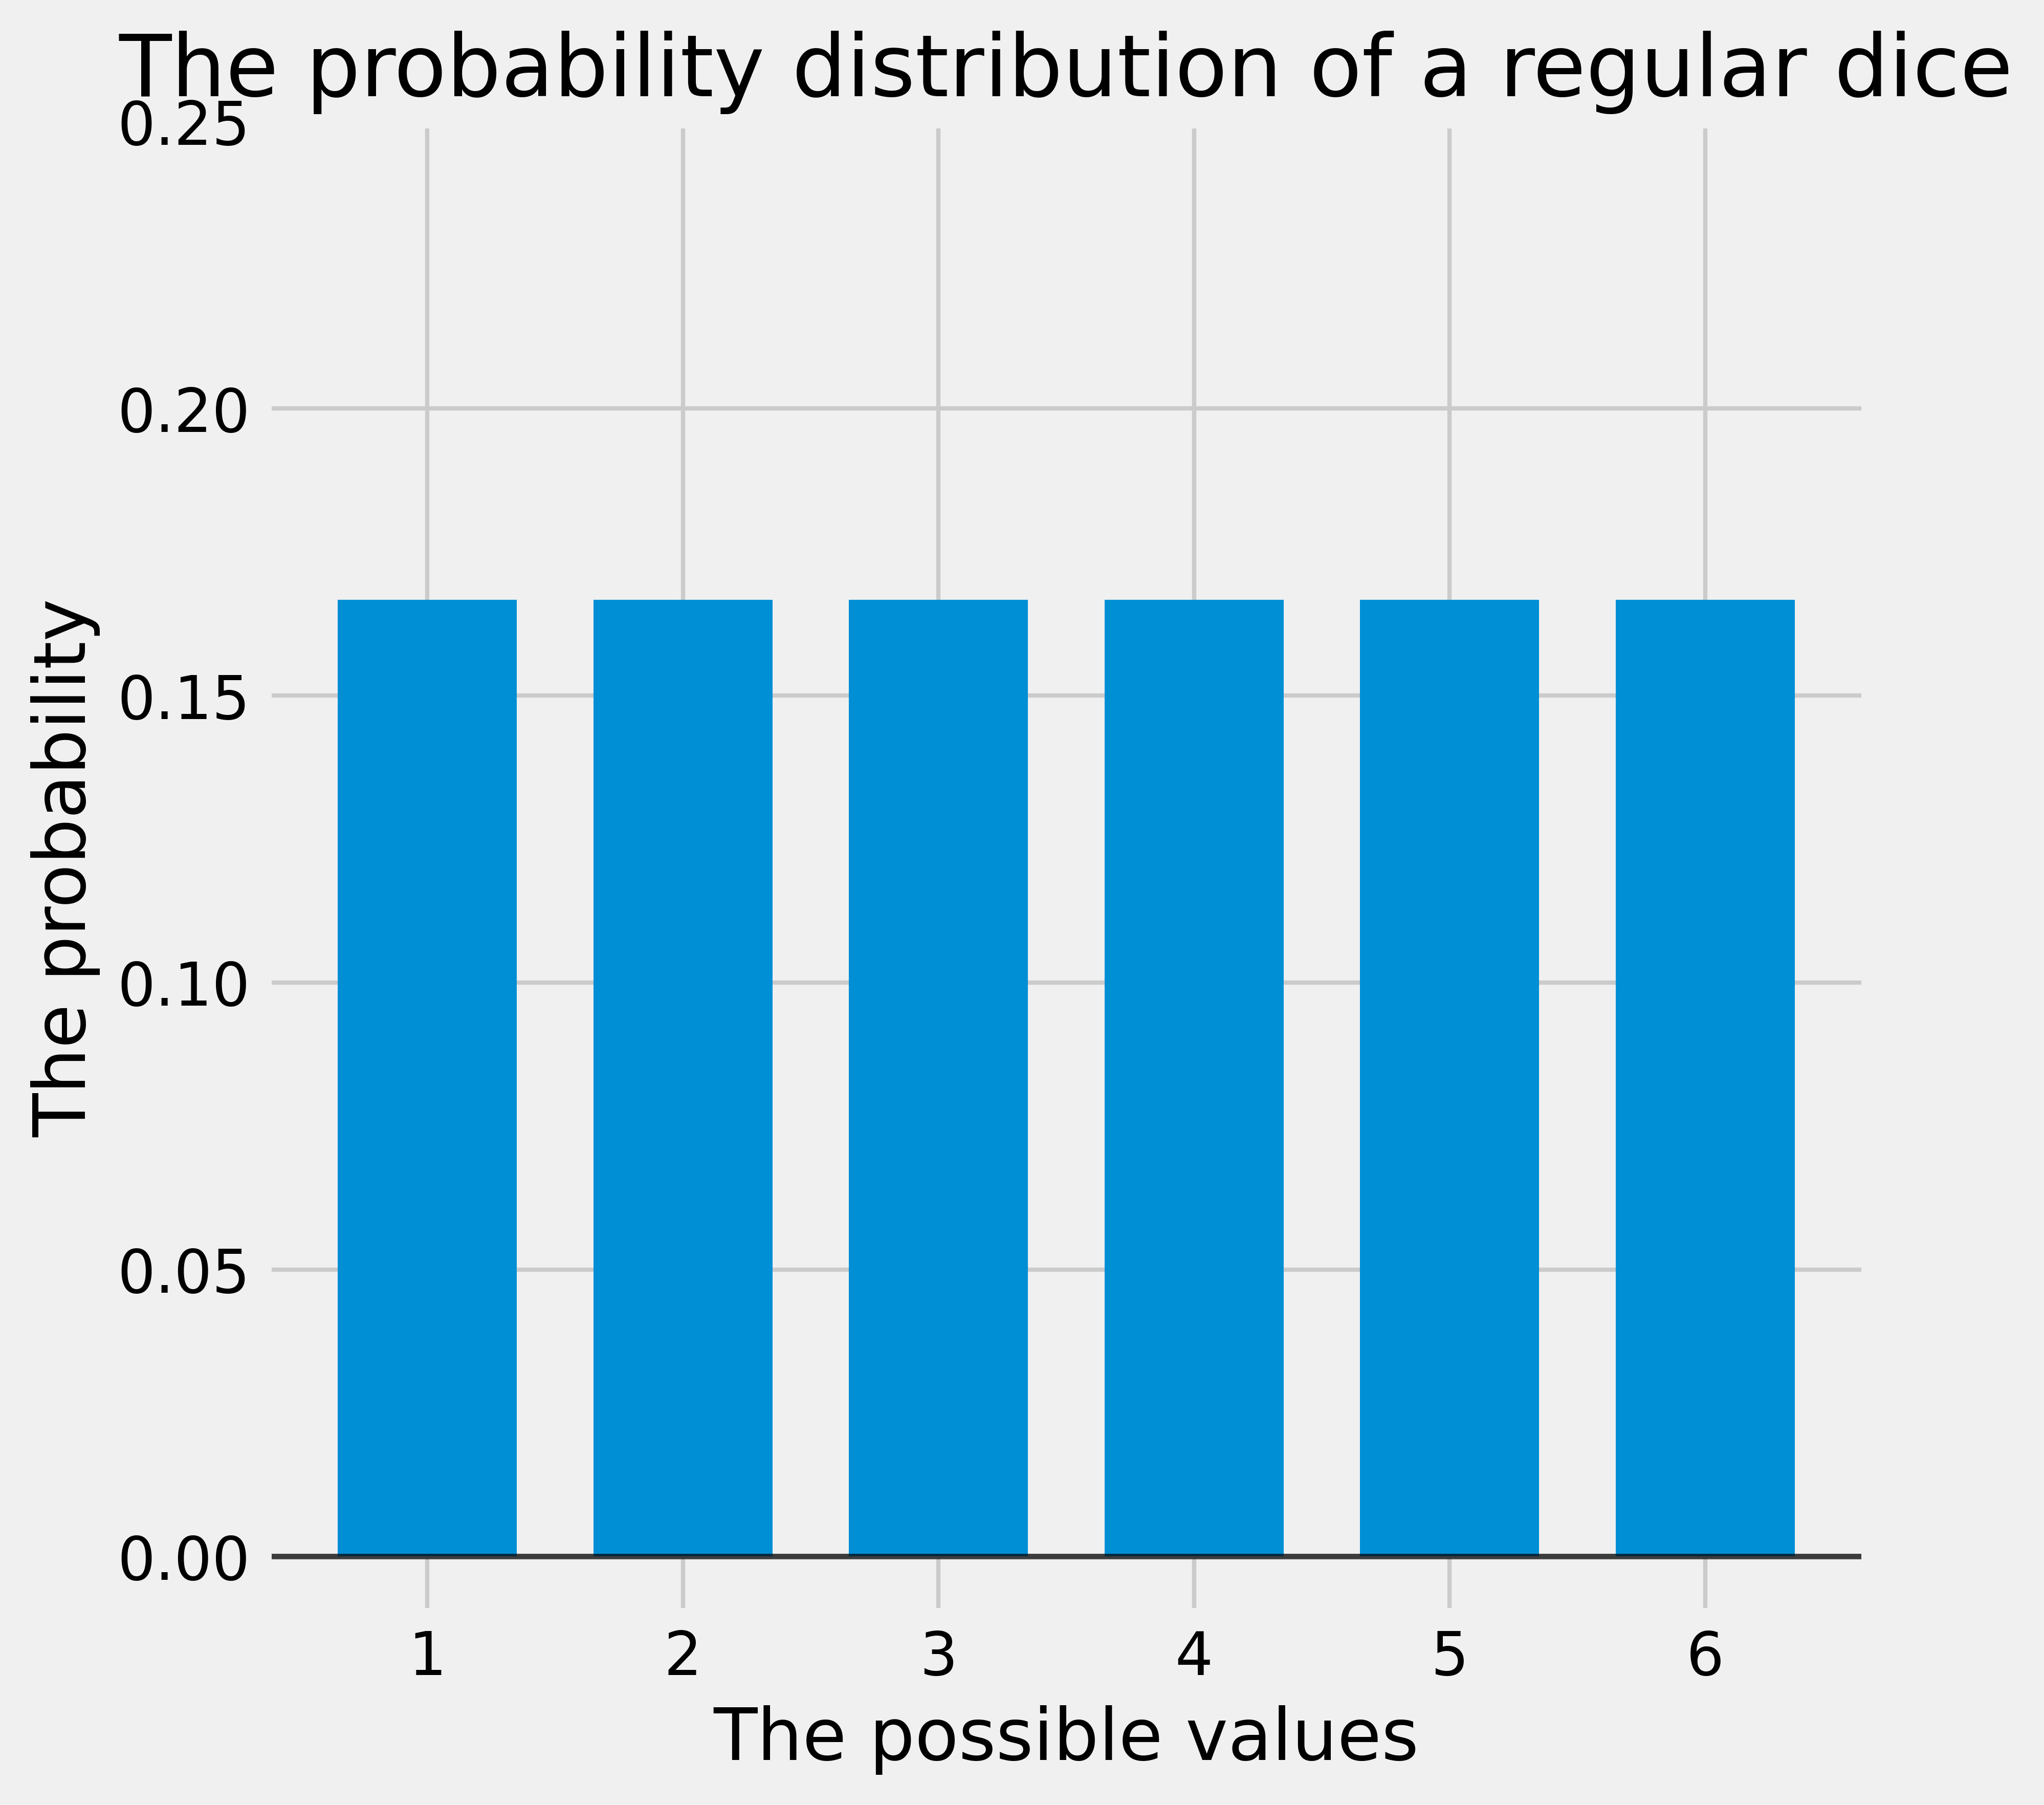
\includegraphics[width=0.43\textwidth,right]{assets/discrete_uniform_pdfs.png}
%    \caption{}
%   \label{fig:discrete_uniform}
%\end{wrapfigure}

%Consider rolling a regular six-sided dice. The side facing up after a roll can take the values from 1 to 6, inclusive, represented by a random variable say $X$. Notice that unless the dice was biased, there is no reason to assume that one value is more probable than the other. In other words, each value of the range of possible values has equal probability of occurrence, precisely $\frac{1}{6}$. The probability can be represented as a distribution as in figure \ref{fig:discrete_uniform}.

%The probability distribution of the random variable $X$ can also be denoted as a discrete uniform distribution. Discrete means the domain is of countable size; uniform means that all possible values have the same probability.

%More formally, the distribution is also defined by its probability function, which is a function mapping a possible value to its chance of occurrence. For our random variable $X$, its probability function $f(X_i)$ is simply:

%\[
%    f(X_i) = \frac{1}{6}
%\]

%But our random variable of likeability does not have a finite domain, I hear you say. The random variable $L$ has infinite values it could take, ranging from zero to one. Thankfully, we can extend our discrete distribution to a continuous distribution.

\begin{wrapfigure}{r}{0.45\textwidth}
    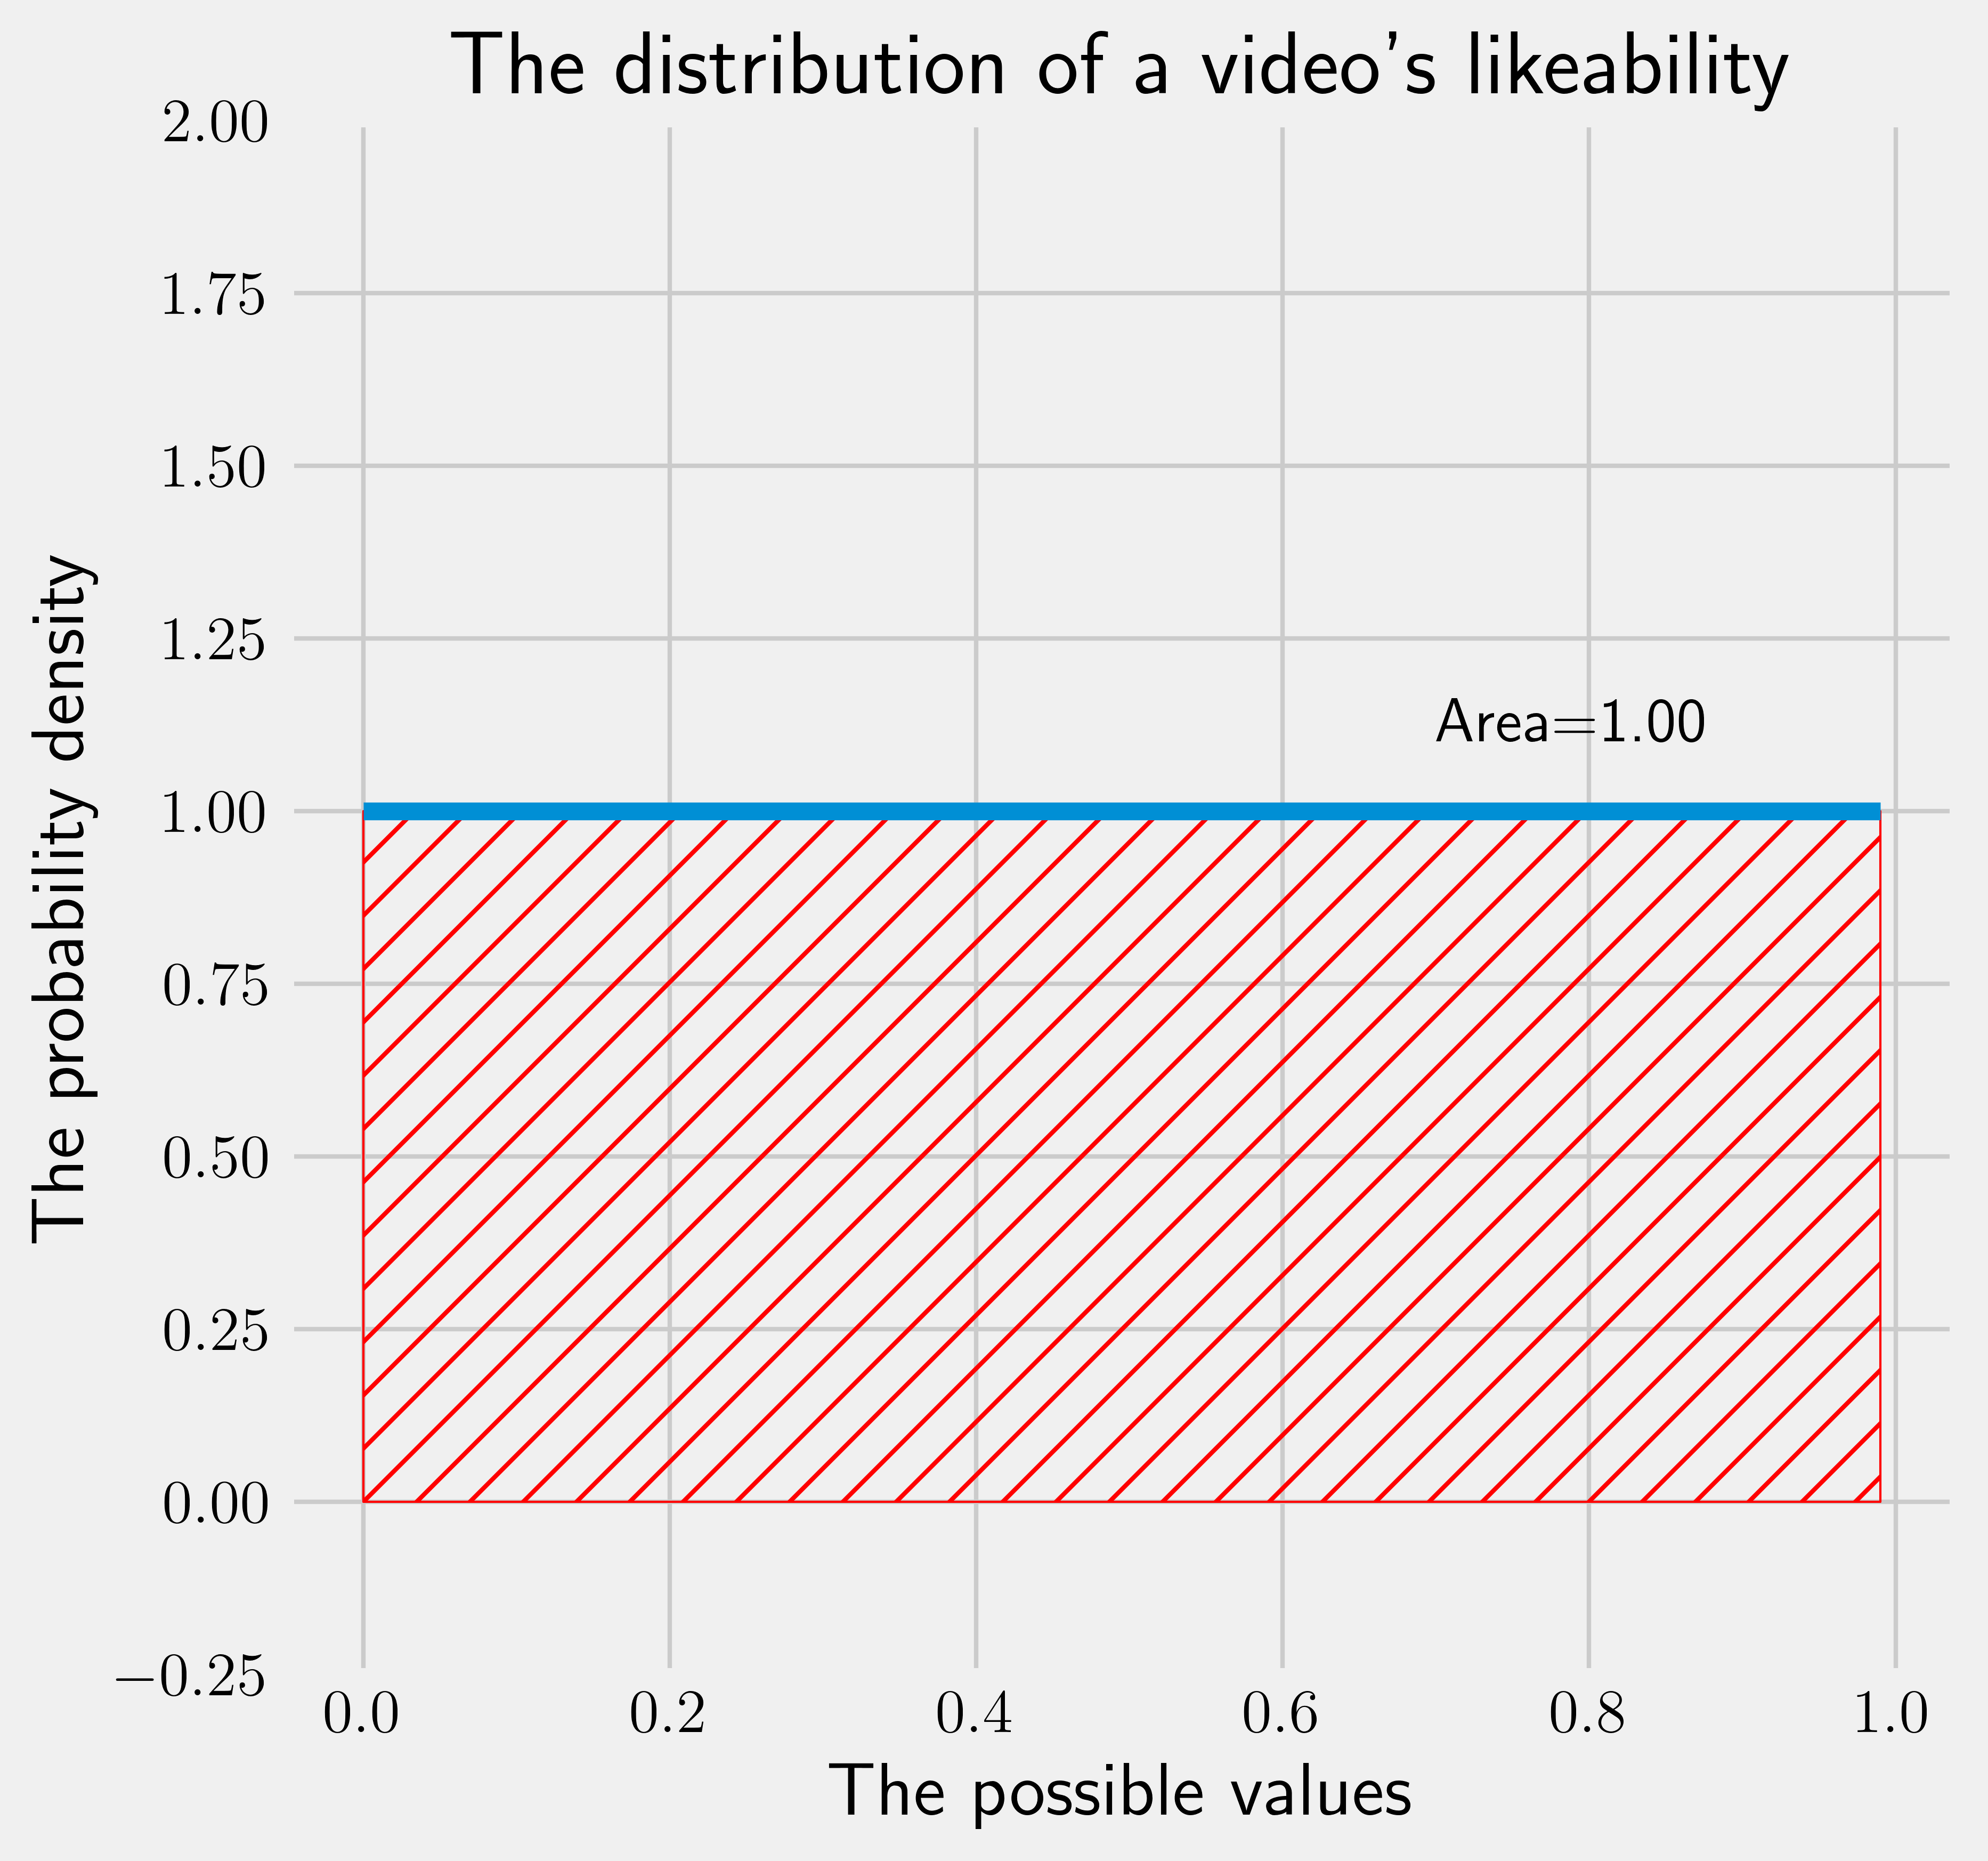
\includegraphics[width=0.43\textwidth,right]{assets/uniform_pdfs.png}
    \caption{}
    \label{fig:uniform}
\end{wrapfigure}

Without any assumptions, the probability density function of a viewer's opinion on a video before they've seen the ratings is a uniform distribution (figure \ref{fig:uniform}). Before seeing the ratings, the likeability $L$ of the video will range continuously from zero to one, but unless the viewer has had a bad day, there is no reason to prefer a range of likeabilities to another. That is, the probability density of a specific likeability value is uniform:
\[
    L \sim U(0, 1).
\]

%However, the y-axis of probabilities must be switched to probably densities, because it is no longer accurate to talk about a specific value's probability --- we must now consider the probability of a range of values instead

Additionally, the area under the probability distribution must be of unit 1. Therefore, the initial probability distribution displayed in figure \ref{fig:uniform} has a probability density function $f(L)$ of:
\[
    f(L) = 1.
\]

Moreover, the statistical mean of this distribution should be initial thought of this unwatched and unrated video. I expect this to be 50\% as there is no reason for me to assume its quality initially --- this is a point that is debated later. Mathematically, the mean $\mu$ of this distribution is:
\begin{align*}
    \mu &= \int_0^1 x \, dx\\
    &= \Eval{\frac{x^2}{2}}{1}{0}\\
    &= 0.5,
\end{align*}
which fulfills this expectations.
%The requirements of continuous distributions restrict the probability distribution of our likeability metric --- it must be positive for all x values in the x-axis domain and have an area of one.

%The uniform distribution of a viewer's prior belief of the likeabilities of a video is an indication of a lack of weighting. Therefore I should not need to add weightings to the statistical mean calculations of the final step.

% the binominal
\subsection{Specific and General Likeability Distributions}
Using the ratings of video one as an example (6 likes and 1 dislike), consider a single likeability value from the domain of the random likeability variable $L$, say 0.5. What is the probability that we see the ratings of video one with a true likeability of 50\%? I decided to use the binomial distribution.

\begin{wrapfigure}{r}{0.45\textwidth}
    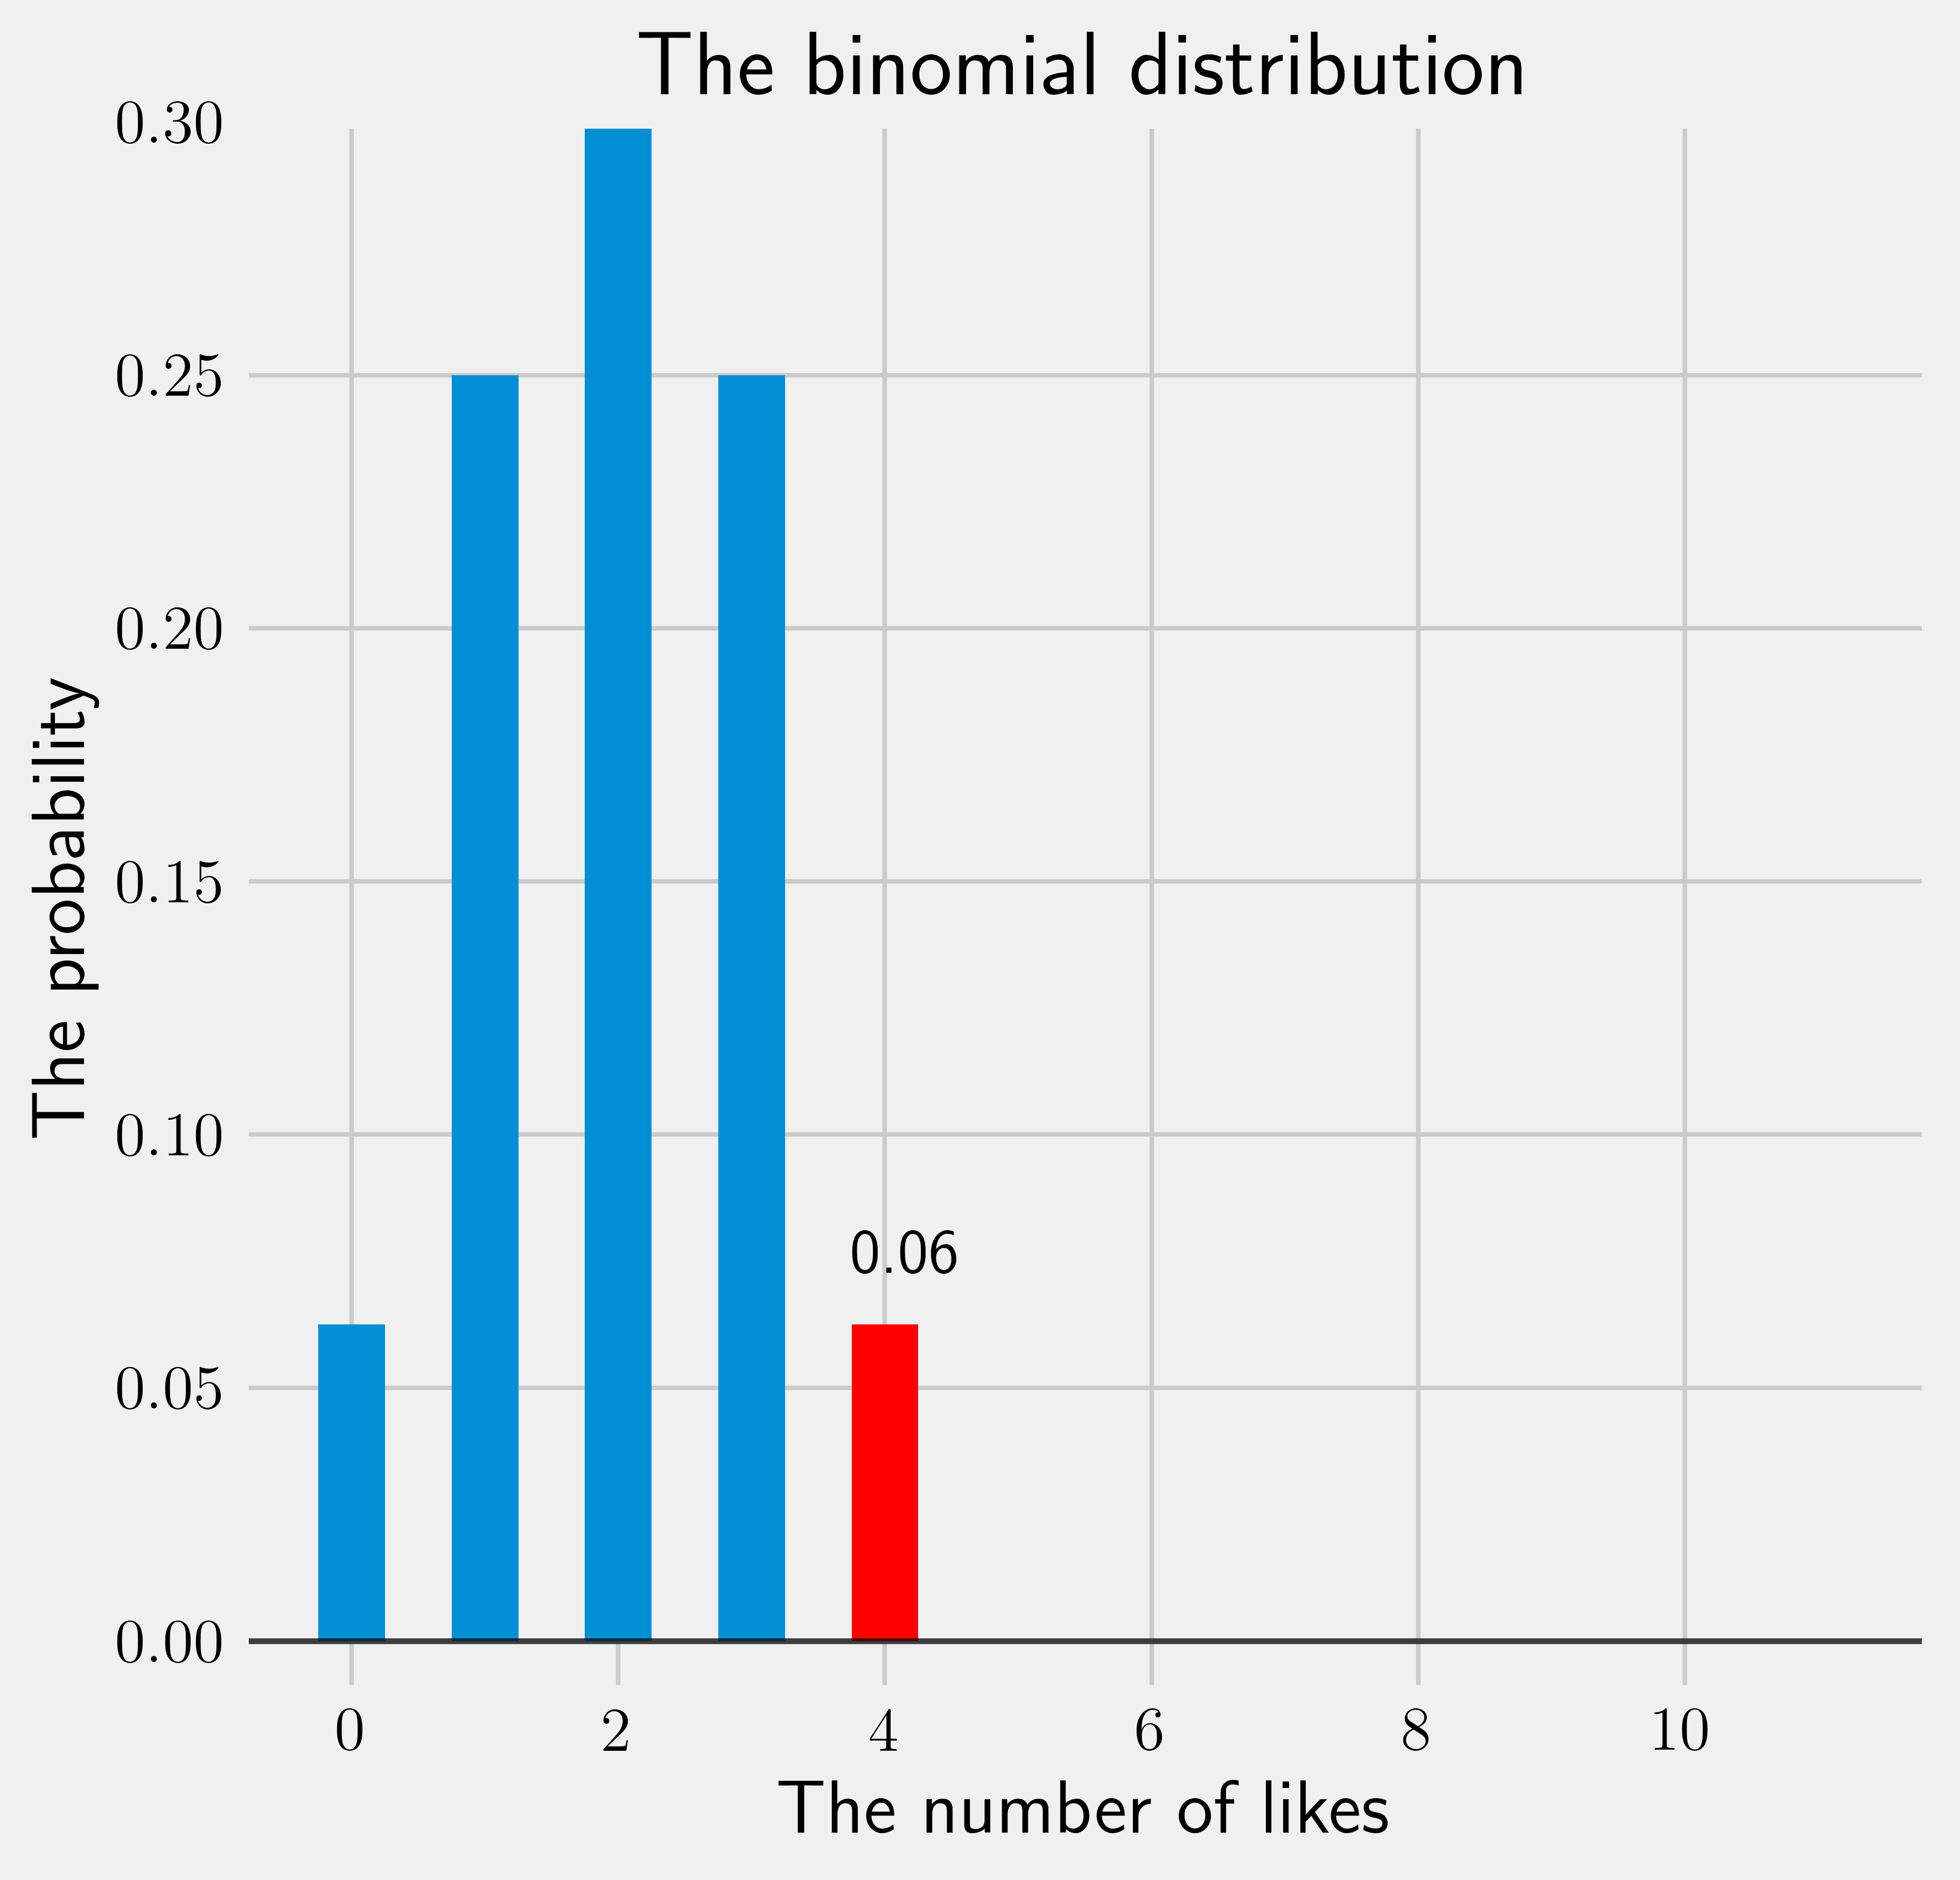
\includegraphics[width=0.43\textwidth,right]{assets/bino_pdfs.png}
    \caption{For video one}
    \label{fig:bino}
\end{wrapfigure}

The binomial distribution is a probability distribution that summarizes the likelihood that a value will take one of two independent values under a given success chance and assumptions \parencite{barone_2021}. In short, the distribution will model the distribution of the number of likes in a sample of ratings given a true likeability. It is a discrete distribution, and its discrete probability distribution function $f(x)$ is of the form:
\[
    f(x) = {n \choose x} p^x (1-p)^{n-x},
\]
where $n$ is the number of ratings, and $p$ is the true likeability of the video. When graphed using the ratings of video one, the distribution resembles that of figure \ref{fig:bino}.

While the distribution displays all the possible likes/dislikes combinations, the value that is of interest is colored in red. The figure shows that the probability of getting 6 likes in 7 ratings is about 0.05 or 5\%. Or as a single calculation:
\[
    f(6) = {7 \choose 6} (0.5)^6 (1-0.5)^{7-6} \approx 0.05.
\]
Therefore for each likeability of our random variable $L$, its probability is $f(6)$ with the variable $p$ replaced by the likeability. Therefore I believe the probability density function $G(l)$ of our random variable is a binomial distribution with parameter $p$ rather than $x$, and is written as:
\[
    G(l) = {n \choose x} l^x (1-l)^{n-x} = {7 \choose 6} l^6 (1-l) ^{7-1}.
\]
where $l$ are the range of likeabilities.

When graphed on software, the likeability distribution looks like the left graph of figure \ref{fig:beta}.

\begin{figure}[H]
    \centering
    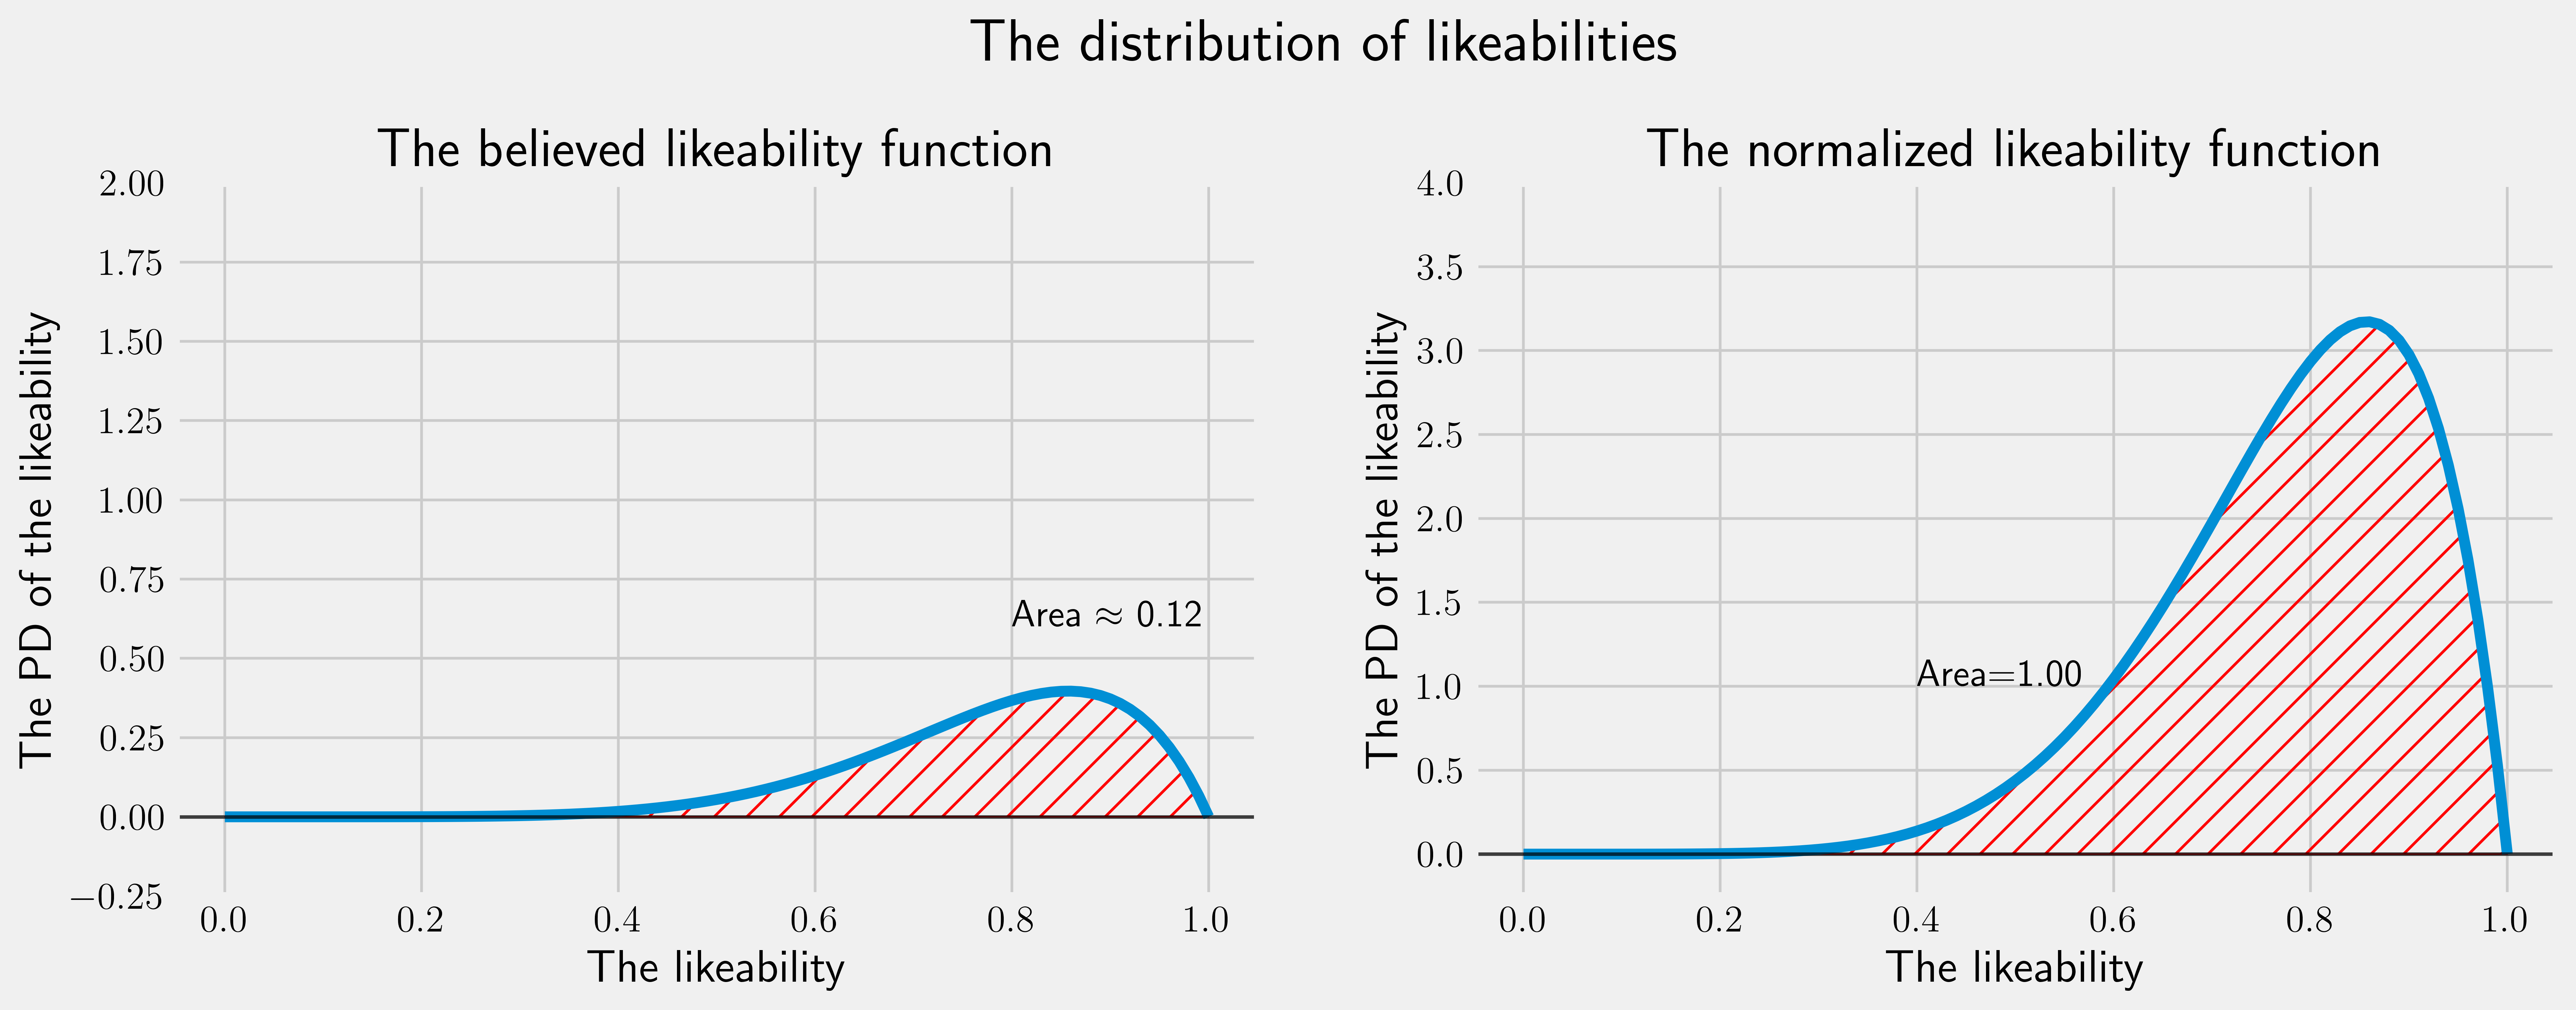
\includegraphics[width=1\textwidth]{assets/beta_pdfs.png}
    \caption{For video one}
    \label{fig:beta}
\end{figure}

The curve plotted by $G(l)$ has a tail towards the left, with a singular peek near the value $0.85$. This corresponded with my simulated likeability distribution.

\subsection{Likeability Distribution Normalization}
But the figure shows that it has an area of only $\approx 0.12$, which does not fit the requirement of a probability density function of area one. I attempted to normalize this distribution by dividing it by its area $A$, that is:
\begin{align*}
    A &= \int_{0}^{1} G(l) \, dl\\
    &= \int_{0}^{1} {n \choose x} l^x (1-l)^{n-x} \, dl\\
    &\approx 0.12.
\end{align*}
Thus I was able to construct the normalized probability density function $K(l)$ for the likeability random variable (shown by the right graph of figure \ref{fig:beta}):
\begin{align*}
    K(l) &= \frac{G(l)}{A}\\
    &= \frac{ {n \choose x} l^x (1-l)^{n-x}} {\int_{0}^{1} {n \choose x} l^x (1-l)^{n-x} \, dl}.
\end{align*}

\subsection{Statistical Mean of Likeability Distribution}
We are now able to take the statistical mean $\mu$ of this function, which would be the statistical solution of the estimated likeability of the video. Notice that we can restrict the integral bounds for the probability density function is only defined between 0 to 1:
\begin{align*}
    \mu &= \int_{-\infty}^{\infty} l K(l) \, dl\\
    &=\int_{0}^{1} l K(l) \, dl\\
    &=\int_{0}^{1} l \frac{ {n \choose x} l^x (1-l)^{n-x}} {\int_{0}^{1} {n \choose x} l^x (1-l)^{n-x} \, dl} \, dl.
\end{align*}

While I was able to reduce the complexity of this integral by canceling the choose function and combining the exponents, the remain integral seems unsolvable to any integration method I know:
\begin{align*}
    \mu &=\int_{0}^{1} \frac{ l^{x+1} (1-l)^{n-x}} {\int_{0}^{1} l^x (1-l)^{n-x} \, dl} \, dl\\
    &= \frac{1}{\int_{0}^{1} l^x (1-l)^{n-x} \, dl} \int_{0}^{1}  l^{x+1} (1-l)^{n-x} \, dl.
\end{align*}

Thankfully, the internet was able to provide me a solution via a special function named the Beta function $B(x,y)$ \parencite{wikipedia_2021} and its relative the Gamma function $\Gamma(z)$ \parencite{artin_2006}, which are defined as:
\begin{align*}
    B(x, y) &= \int_{0}^{1} l^{x-1} (1-l)^{y-1} dl\\
    \Gamma(z) &= \int_{0}^{\infty} x^{z-1} e^{-x} \, dx.
\end{align*}

To put it simply, the Gamma function is an analytic continuation of the factorial operation --- meaning that it generalizes the factorial operation outside the positive integers. It has two relevant identities. The first states its relation with the factorial operation, the second showing its identity with the Beta function:
\begin{align*}
    \Gamma(z) &= (z-1)!\\
    B(x, y) &= \frac{\Gamma(x) \Gamma(y)}{\Gamma(x + y)}.
\end{align*}

I was able to simplify the formula for the statistical mean using the Beta function, which can be converted to a series of Gamma functions and therefore into factorials:
\begin{align*}
    \mu &= \frac{1}{B(x+2, n-x+1)}B(x+1, n-x+1)\\
    &= \frac{\frac{\Gamma(x+2)\Gamma(n-x+1)}{\Gamma(n+3)}}{\frac{\Gamma(x+1)\Gamma(n-x+1)}{\Gamma(n+2)}} =  \frac{\frac{(x+1)!(n-x)!}{(n+2)!}}{\frac{x!(n-x)!}{(n+1)!}}\\
    &= \frac{x+1}{n+2} = \frac{6+1}{7+2} \approx 0.778.
\end{align*}

It was surprising how neat the final solution was given the complexity that is the integral beforehand. Furthermore, this shows that the statistical likeability of the video can be calculated by dividing the number of likes plus one over the number of ratings plus two, under the assumption that the initial likeability distribution was uniform.

\subsection{Method Analysis}
The small difference between the statistical method and the simulation method ($|0.776 - 0.778| = 0.002 \approx 2.58\%$) showcases not only the correctness of this solution, but it also illustrates the power of simulations --- I did not have to do any maths to get an approximate answer. However, this neat solution explains the validity of the naive method at large rating numbers, for the plus ones and twos become insignificant as their operands increases.

Overall, the statistical method required a reasonable amount of statistical knowledge, and I was greatly assisted by the use of a computer program in checking the equalities between each simplifying step. However, it produced a tidy result that is easy to remember and fast to compute. Table \ref{tbl:stat} lists the five videos ranked by their statistical likeability.

\begin{figure}[H]
    \centering
    \begin{tabular}{c|c|c|c|c|c}
        & Video A & Video B & Video C & Video D & Video E \\
        \hline
        \hline
        Statistical Likeability (3dp) & 0.833 & 0.926 & 0.854 & 0.941 & 0.994
    \end{tabular}
    \captionof{table}{}
    \label{tbl:stat}
\end{figure}

\section{Bayesian Approach}
The premise of this section was hinted upon within the statistical analysis of the probability distribution of the likeability random variable. I am going to break the premise of the uniform prior probability density function. The myriads of reasons include: YouTube recommendations are algorithmic and is unlikely to recommend me a low likeability video; it is very difficult to make a poor maths video on a topic, for I believe the subject has a high skill ceiling of entering; and personally, I enjoy watching these maths videos online, and have slightly higher expectations of the community. While these factors are difficult to capture in traditional statistical distribution analysis, it is the core idea in a branch of statistics called Bayesian statistics.

% frequenist, bayesian
The core principles in the two branches of statistics differ in their interpretations of probabilities. The frequentists define the probability by its percentage of occurrence as the sample size increases to infinity, with the manipulations of random variables being convolutions; the Bayesians perceive probabilities as a belief of the next event, which updates as new data are seen. The method of combining binomial and uniform distributions fits the frequentists view, but the Bayesian view perfectly fits my requirement of a changeable initial belief.

% set up, definitions
\subsection{Defining the Bayesian Prior, Posterior, and Event}
Consider the random variable likeability $L$ of the video. Its probability density function $P(l)$ represents a belief in the likeability of the video given all data available. Before seeing any new data, this function is called the Prior. The arrival of new data is denoted by the symbol $D$, and the updated likeability upon seeing the new data is denoted by $P(l | D)$ --- the probability density function of the likeability \textit{given} the new data. This updated likeability is called the Posterior. In the context of video ratings, the prior probability will denote my initial belief on the likeabilities of the video, to which I can update my prior upon every new rating I see. I will define the Bayesian likeability to be the statistical mean of the prior.

%To find the relations between the prior and posterior probabilities, we can use the example of a medical test of a common illness.

%\begin{wrapfigure}{r}{0.45\textwidth}
%    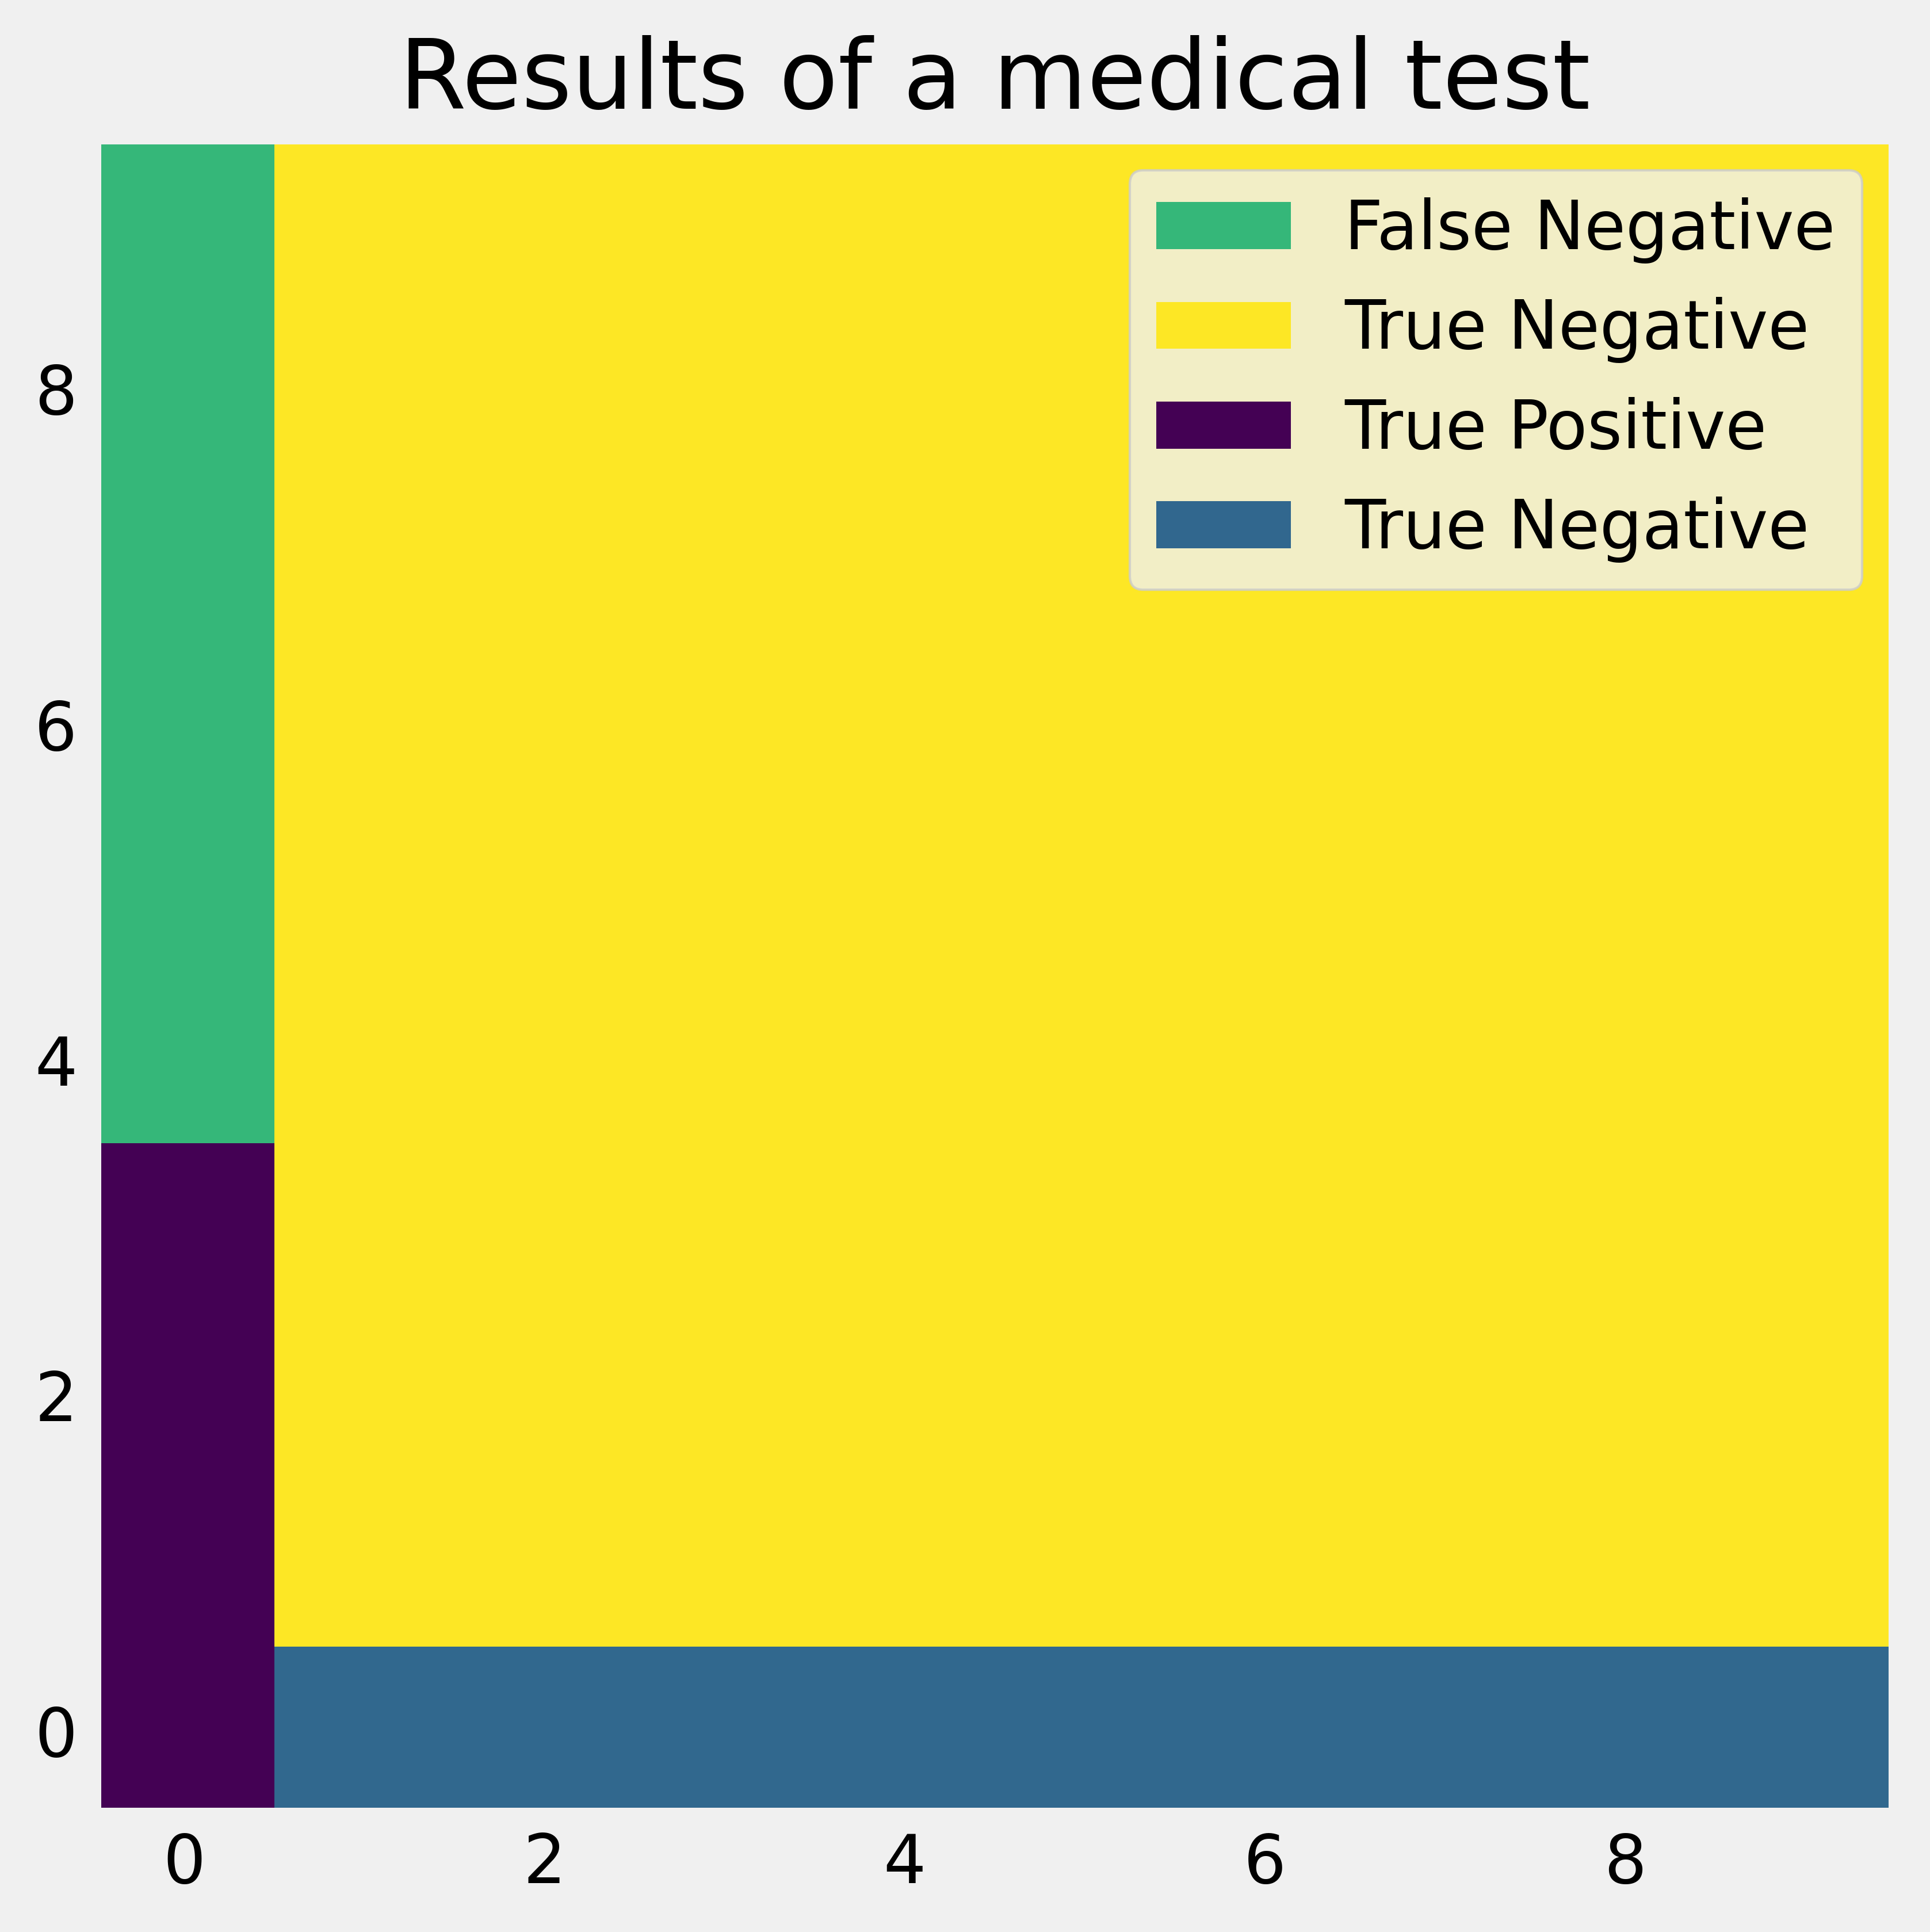
\includegraphics[width=0.43\textwidth,right]{assets/medical_scenario.png}
 %   \caption{}
 %   \label{fig:medical}
%\end{wrapfigure}

%Assuming we are faced with a patient showing no symptoms, but had taken a test of the common illness (0.1 probability of occurrence) which is positive with a sensitivity of 0.4 and a specificity of 0.9 --- meaning that there is a 40\% chance the test is positive if the patient actually has the illness; and a 90\% chance that the test is negative if the patient actually lacks the illness. Our prior beliefs before seeing the test result rely on the average chance that a random person in the area has the illness, or 10\%. The situation is shown in figure \ref{fig:medical}.

%For the posterior is our beliefs after seeing the positive test result, it is calculated by the probability of the patient being ill and having a positive test result, divided against the probability of a person being positive no matter their situation. This can be expressed by a formula:
%\[
  %  \text{Posterior} = \frac{P(\text{Ill} \,\text{and}\, \text{Positive})}{P(\text{Whatever and Positive})}
%\]

%The notation of the probability of $A$ and $B$ is defined by the probability of $A$ times the probability of $B$ given $A$ is true. And by substituting for the symbols $P(x)$ for the probability of illness, we have found Bayes Theorem:
The regular Bayes theorem for updating scalar probabilities should be familiar:
\begin{align*}
    P(x|D) &= \frac{P(D|x) P(x)}{\sum P(D|x_i) P(x_i) }\\
     &= \frac{P(D|x)P(x)}{P(D|x)P(x) + P(D|\neg x)P(\neg x)},
\end{align*}
where $x$ is the prior belief of some event, and $x_i$ representing the space of all possible events.

%More specifically, the probability of illness $P(x)$ is simply the prior of illness, which is $0.1$; the probability of a positive test result given the illness $P(D|x)$ is the sensitivity of the test, or $0.4$; and the probability of a positive test result is the sum of having and not having the illness, multiplied by their respective chance of testing positive, or $0.4 \times 0.1 + (1- 0.9) \times (1-0.1)$. In our medical example, the updated belief on the probability of illness upon seeing a positive test result is thus:
%\begin{align*}
%    P(x|D) &= \frac{0.4 \times 0.1}{0.4 \times 0.1 + (1-0.9) (1-0.1)}\\
%    &\approx 0.308
%\end{align*}
%Our belief of the probability of illness of the patient had been updated from $0.01$ to $0.308$. While it is reasonable that a positive test result conveys a higher chance of illness, it still really surprised me when I first saw it. How is it that we can only be 31\% sure of the illness if the test has an accuracy of 40\%? This discrepancy with naive solutions is also present in the naive likeability method, which may be a warning that special care is needed to tread in the field of statistics --- especially if one may be diagnosing a patient wrongly.

% actual attempt
I would need to extend this theorem to fit our continuous belief of the likeabilities of a video. To check for the validity of this method, I will be first applying the extended method on an uniform prior.

\subsection{Prior Updating and the Continous Bayes Theorem}
With the random variable likeability $L$, the initial prior $P(l)$ of the likeability is a continuous uniform distribution:
\[
    P(l) = 1.
\]

Let's consider the likeability posterior $P(l|D)$ given the new data $D$ of seeing a like on the video. By Bayes Theorem, the likeability distribution after seeing a like on the video is:
\begin{align*}
    P(l|D) &= \frac{P(D|l) P(l)}{\sum P(D|l_i) P(x_i) }.
\end{align*}

Because we are now dealing with a functional prior and posterior (of parameter likeability), all of the probabilities in the equation will be functions and the summation must be switched to integrals. Therefore I was able to rewrite the discrete Bayes Theorem into a continuous version (the $\theta$ symbol is used to differentiate between the function parameter and the likeability random variable ):
\[
    P(l|D)(\theta) = \frac{P(D|l)(\theta) \times P(l)(\theta)}{\int_{0}^{1} P(D|l)(\theta) \times P(l)(\theta) \, d\theta},
\]
note the integral on the denominator has bounds zero to one, inclusive, for that is the domain of the prior likeability random variable.

The probability of seeing one like given a specific likeability is the likeability from definition:
\[
    P(D|l)(\theta) = \theta.
\]

Therefore after substitution, the equation simplifies and can be solved:
\begin{align*}
    P(l|D)(\theta) &= \frac{\theta \times 1}{\int_{0}^{1} \theta \times 1 \, d\theta}\\
    &= \frac{\theta}{\int_0^1 \theta \, d\theta}\\
    &= \frac{\theta}{\Eval{\frac{\theta^2}{2}}{1}{0}}\\
    &= 2\theta.
\end{align*}

\newpage
The posterior probability density function of the likeability of a video is $2\theta$ given a prior uniform distribution of $1$. The statistical mean $\mu$ of this function can also be calculated to be around $66\%$.
\begin{align*}
    \mu &= \int_0^1 \theta P(l|D)(\theta) \, d\theta\\
    &= \int_0^1 2\theta^2 \, d\theta\\
    &= \Eval{\frac{2\theta^3}{3}}{1}{0}\\
    &= \frac{2}{3}.
\end{align*}

The statistical mean of a video with 1 like and no dislikes by the statistical method also agree to this value, showing the validity of the Bayesian method for the first like.
\begin{align*}
    \mu &= \frac{x+1}{n+2}\\
        &= \frac{2}{3}
\end{align*}

\subsection{N-Likes Generalization}
I thought to generalize this by seeing what happens as the prior is updated $n$ times with $n$ likes only. Consider a prior probability density function at the $n$th like of the form:
\[
    P(l)(\theta) = A \theta^B,
\]
where $A$ and $B$ are constants. Our initial prior is achieved by setting $A=1$ and $B=0$.

Therefore the unknown probabilities are:
\begin{align*}
    P(D|l) &= \theta\\
    P(D) &= \int_0^1 \theta A\theta^B \, d\theta,
\end{align*}

and the posterior can be represented by:
\begin{align*}
    P(\theta|D) &= \frac{\theta A\theta^B}{\int_0^1 \theta A\theta^B \, d\theta}\\
    &= \frac{\theta^{B+1}}{\int_0^1 \theta^{B+1} \, d\theta}\\
    &= \frac{\theta^{B+1}}{\Eval{\frac{\theta^{B+2}}{B+2}}{1}{0}}\\
    &= (B+2) \theta^{B+1}.
\end{align*}

Because the posterior is of the same form as the prior, the cycle can continue where $A_{n+1} = B_{n}+2$ and $B_{n+1} = B_n+1$, and so $B_n$ denotes the nth like received, and $A_n$ is one above $B_n$. The statistical mean $\mu_n$ of each posterior $B_n$ are:
\begin{align*}
    \mu_n &= \int_0^1 \theta A_n \theta^{B_n} \, d\theta\\
    &= \int_0^1 A_n \theta^{B_n + 1} \, d\theta\\
    &= A_n \Eval{\left(\frac{\theta^{B_n+2}}{B_n+2}\right)}{1}{0}\\
    &= \frac{A_n}{B_n+2}\\
    &= \frac{B_n+1}{B_n+2} = \frac{n+1}{n+2}.
\end{align*}

Once again, this generalization states the Bayesian likeability is the increment of the number of likes divided by the total amount of ratings plus two. This matches the result from the statistical method, albeit with a very different perspective on probabilities and new information. I believe this updating of priors is more appreciated when graphed --- figure \ref{fig:up} showcases the priors of three consecutive likes on a video. Notice how the most likes seen, the less likely the lower likeability values are to occur and the more likely the higher likeability values are to occur.

\begin{figure}[H]
    \centering
    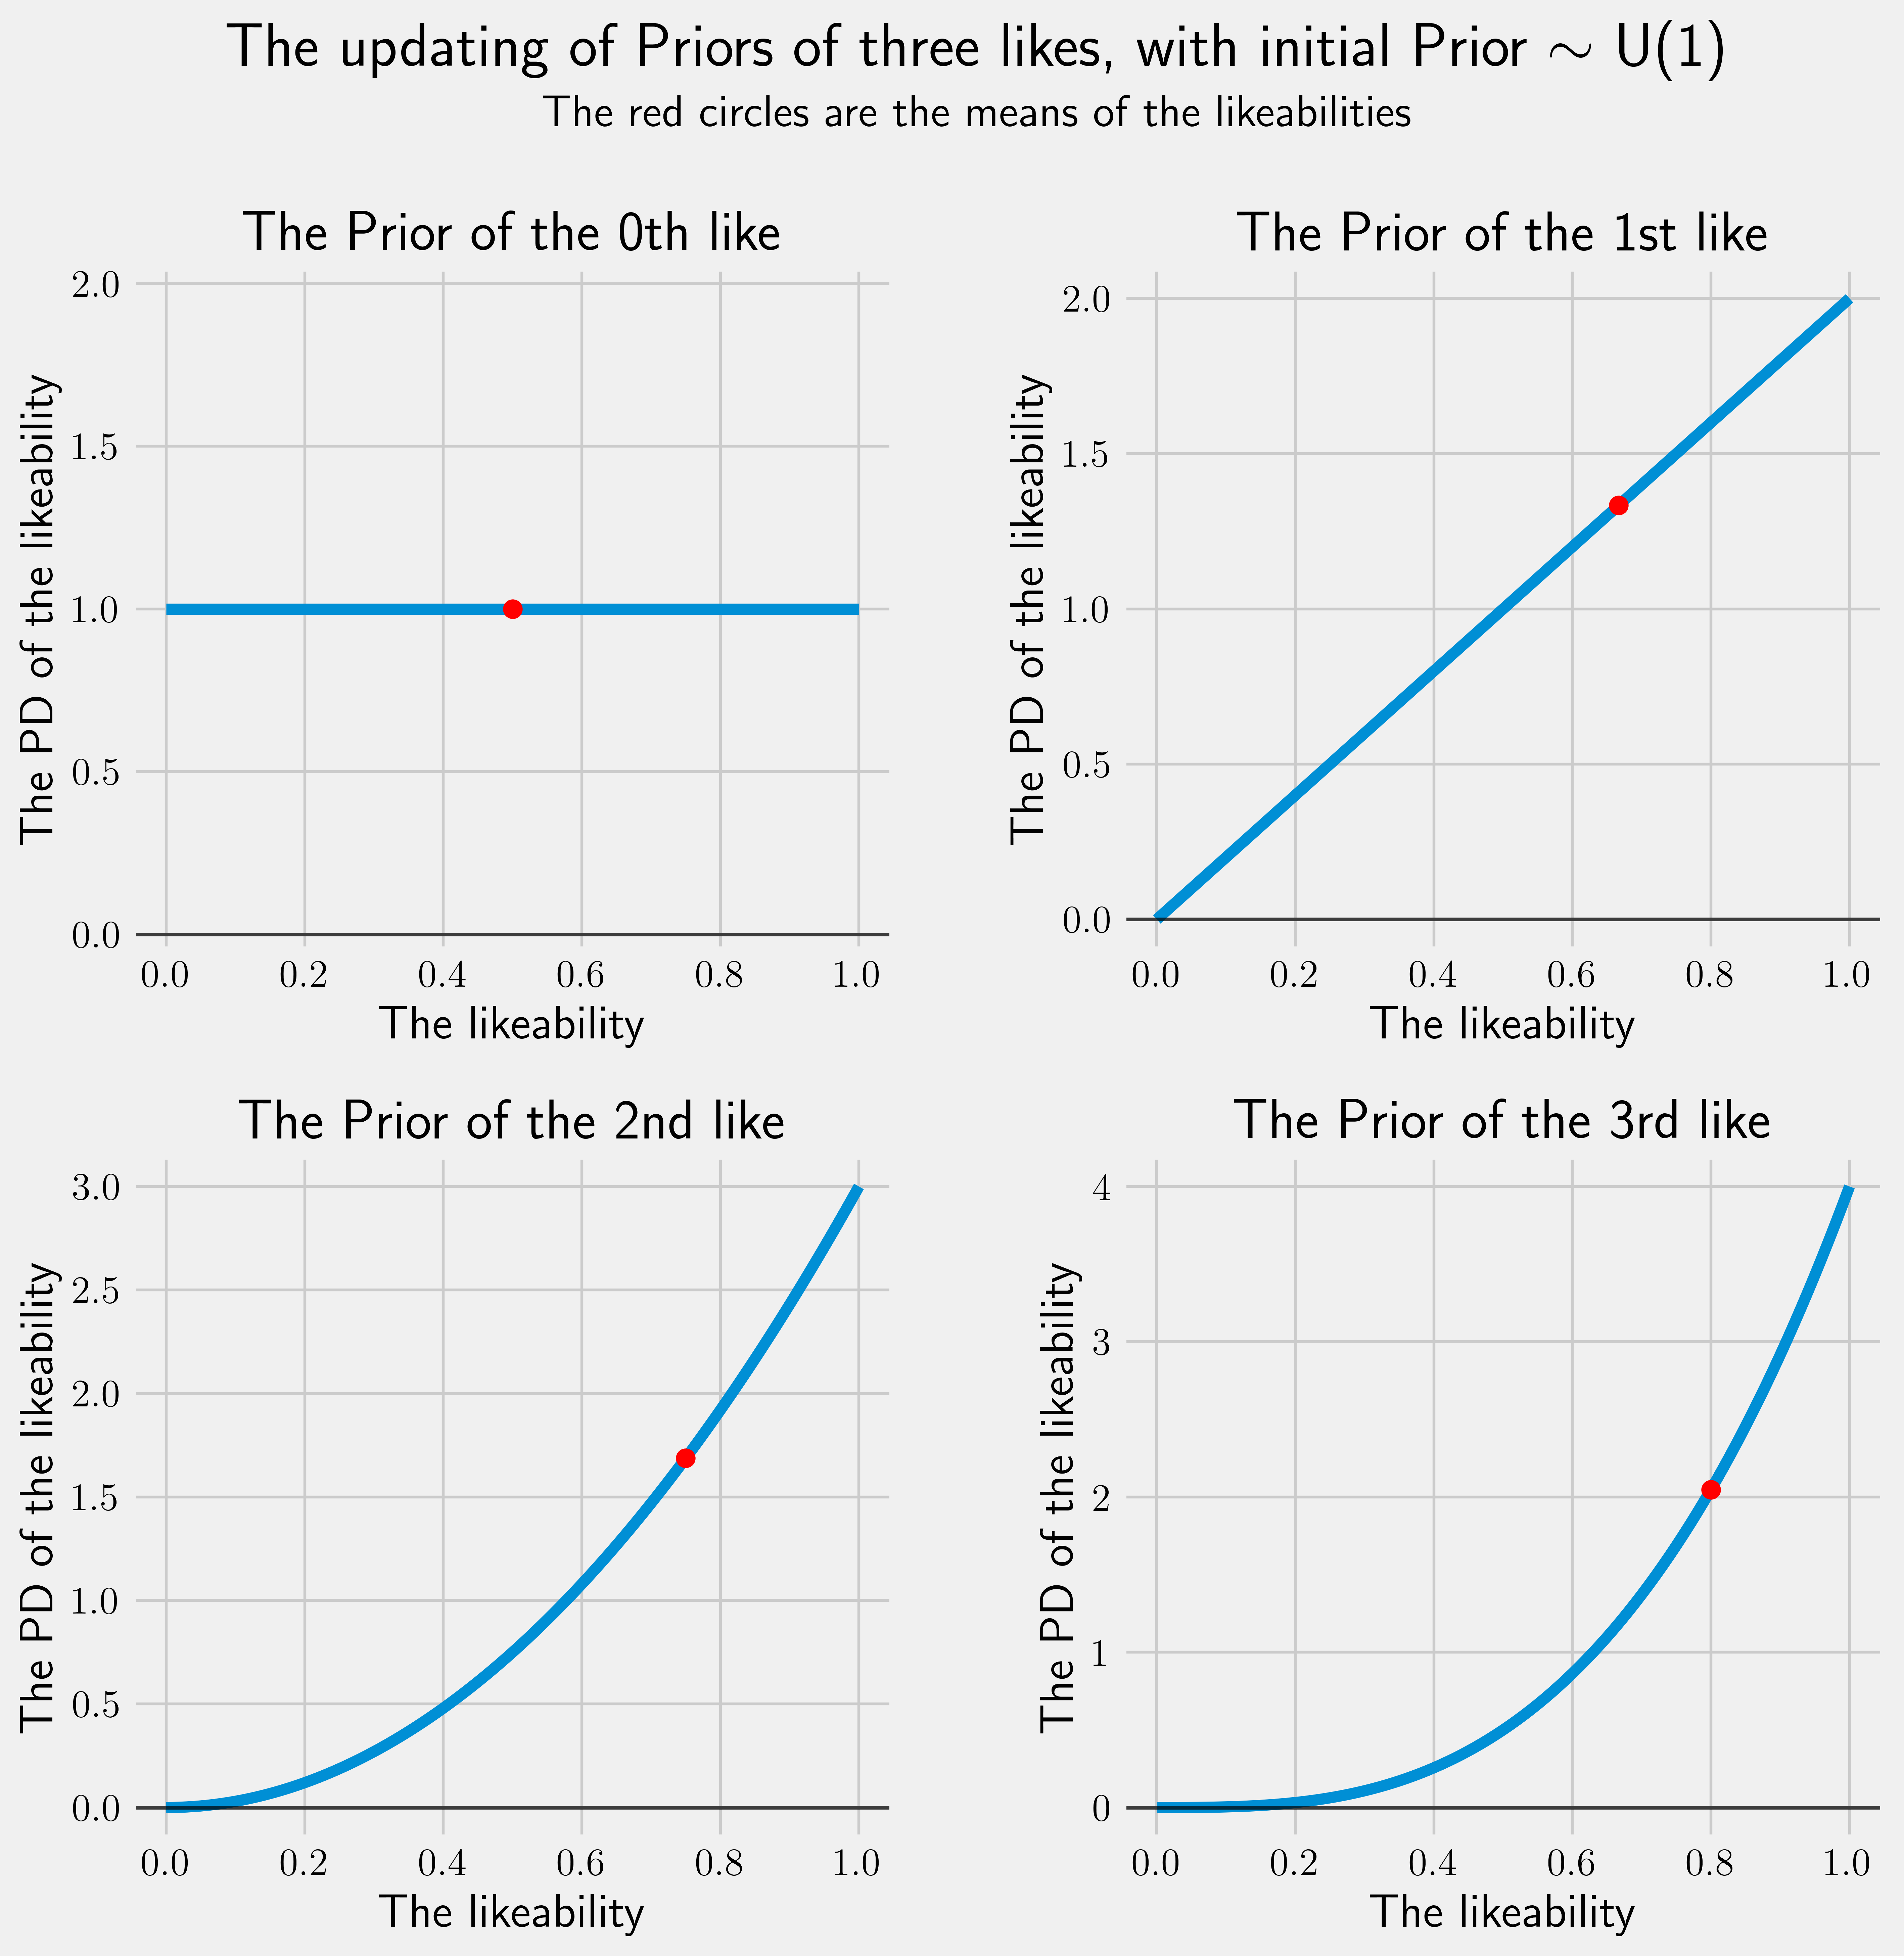
\includegraphics[width=0.7\textwidth]{assets/updating_priors.png}
    \caption{}
    \label{fig:up}
\end{figure}

\subsection{X-Likes Y-Dislikes Generalization}
To generalize the likeability solution to both likes and dislikes, consider the variable $R$ to be the event of seeing $X$ likes and $Y$ dislikes on a video. The posterior originating from a uniform prior is:
\[
    P(l|R)(\theta) = \frac{P(R|l)(\theta) P(l)(\theta)}{\int_0^1 P(R|l)(\theta) P(l)(\theta) \, d\theta}.
\]

The probability of seeing $X$ likes and $Y$ dislikes given a likeability $\theta$ is determined by the binomial distribution:
\[
    P(R|l)(\theta) = {X+Y \choose X} \theta^X (1-\theta)^Y.
\]

Therefore by substitution, we see a familiar form of the posterior:
\begin{align*}
    P(l|R)(\theta) &= \frac{1}{\int_0^1 {X+Y \choose X} \theta^X (1-\theta)^Y P(l)(\theta)\,d\theta}{X+Y \choose X} \theta^X (1-\theta)^Y P(l)(\theta)\\
    &= \frac{1}{\int_0^1 \theta^X (1-\theta)^Y \,d\theta} \theta^X (1-\theta)^Y.
\end{align*}

By letting the variable $n=X+Y$ and $x=X$, this is the exact probability density function from the statistical method. As that method has shown using Beta and Gamma functions, the statistical mean $\mu$ of the posterior probability density function is of the form:
\begin{align*}
    \mu &= \frac{x+1}{n+2}\\
    &= \frac{X+1}{(X+1) + (Y+1)}.
\end{align*}

More importantly, we can also see the Bayesian likeability of a uniform prior can be computed similarly to the naive method of percentages, but adding one to the number of likes and dislikes. It presents an even more handy rule to calculate the mean likeability --- use the naive method with the number of likes plus one and the number of dislikes plus one. The tables of videos A to E are not displayed here for the values are the same as the statistical method.

\subsection{Personal Square-root Prior}
Because of the Bayesian method, we are now freely able to switch out the prior probability density function. As the five videos I've sampled are from the recommendations of YouTube, and they are of a topic which I enjoy --- about mathematics, my initial prior ideally should be higher in probability with higher likeabilities, and has a statistical mean higher than 0.5, as well as fitting all attributes of a statistical distribution.

There is a function I've encountered in class when learning about inverse functions, the absolute of the square root of $x$, $|\sqrt{x}|$. The function is the positive values of the inverse function $x^2$ restricted by the domain from zero to one, inclusive, which from now would simply be referred to as the square root function. It is shown on the left graph in figure \ref{fig:sqrt_per}.

\begin{figure}[H]
    \centering
    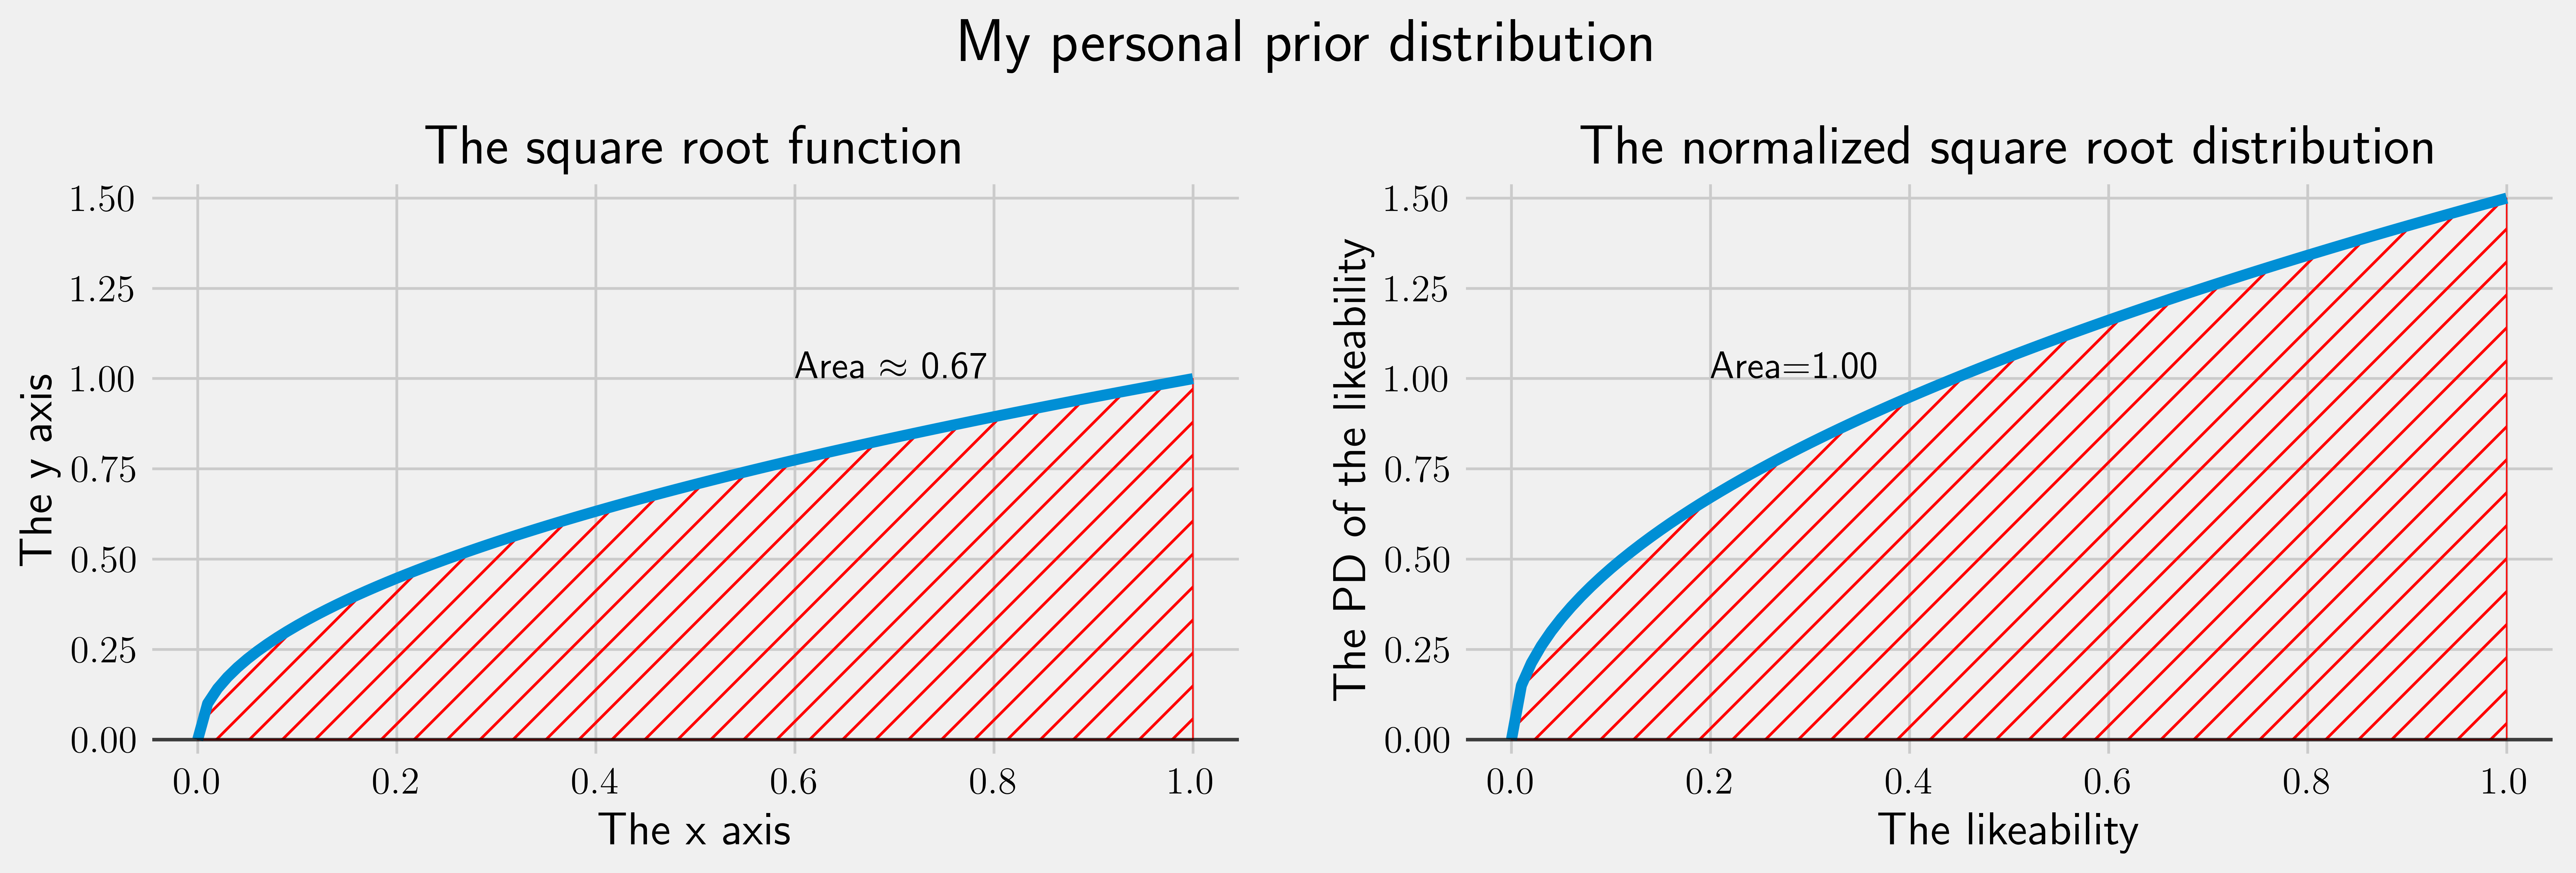
\includegraphics[width=\textwidth]{assets/sqrt_per.png}
    \caption{}
    \label{fig:sqrt_per}
\end{figure}

The function has a decreasing positive slope throughout the domain, meaning that while higher likeabilities are more probable, the rate at which this increases is decreasing so that I am not heavily favoring these videos. However, it needs to be normalized $\text{nsqrt}(x)$ for the area it encloses is less than one.

We can simply scale the function down by the area $A$ it encloses:
\begin{align*}
    A &= \int_0^1 \sqrt{x} \, dx\\
    &= \Eval{\frac{x^{\frac{3}{2}}}{\frac{3}{2}}}{1}{0}\\
    &= \frac{2}{3}.
\end{align*}

Therefore I've defined the normalized square-root function to be:
\begin{align*}
     \text{nsqrt}(x) &= \frac{\sqrt{x}}{A}\\
    &= \frac{3}{2} \sqrt{x}.
\end{align*}

The statistical mean $\mu$ of the normalized square root function also plays nicely, for it is above 0.5, corresponding to my initial high expectations of these videos.
\begin{align*}
    \mu &= \int_0^1 x \frac{3}{2} \sqrt{x} \, dx\\
    &= \frac{3}{2} \int_0^1 x^{\frac{3}{2}} \, dx\\
    &= \frac{3}{2} \Eval{\left(\frac{x^{\frac{5}{2}}}{\frac{5}{2}}\right)}{1}{0}\\
    &= \frac{3}{5} = 0.6.
\end{align*}

Using the normalized square root function as the prior, the posterior probability density function $P(l|R)$ for event $R$ of $X$ likes and $Y$ dislikes is computed by:
\begin{align*}
    P(l|R) &= \frac{1}{\int_0^1 \text{nsqrt}(\theta) \theta^X (1-\theta)^Y } \text{nsqrt}(\theta) \theta^X (1-\theta)^Y.
\end{align*}

This integral is extremely difficult to compute analytically, for there is a non-constant term inside the Beta function, but I was able to integrate it using software and generate a numerical solution. Figure \ref{fig:up_nsqrt} shows how the nsqrt prior updates for three consecutive likes on a video.

\begin{figure}[H]
    \centering
    
\includegraphics[width=0.7\textwidth]{assets/nsqrt_updating_priors.png}
    \caption{}
    \label{fig:up_nsqrt}
\end{figure}

Therefore the Bayesian likeability of video one is numerically computed to be $\approx 0.789$. This is slightly higher than the statistical likeability of $0.778$, reflecting how I had initial high expectations expressed by the nsqrt prior probability density function.

Furthermore, it seems that not only there is no difference between treating the event seeing $X$ likes and $Y$ dislikes as one event $R$, or as multiple updates of events $D$ of one like or dislike, the order of likes and dislikes when sequentially updating also does not impact the final Bayesian likeability. This is shown in figure \ref{fig:nsqrt_incre} where the mean likeability is plotted against the nth rating for three ways of achieving the ratings of video one (6 likes and 1 dislike).

\begin{figure}[H]
    \centering
    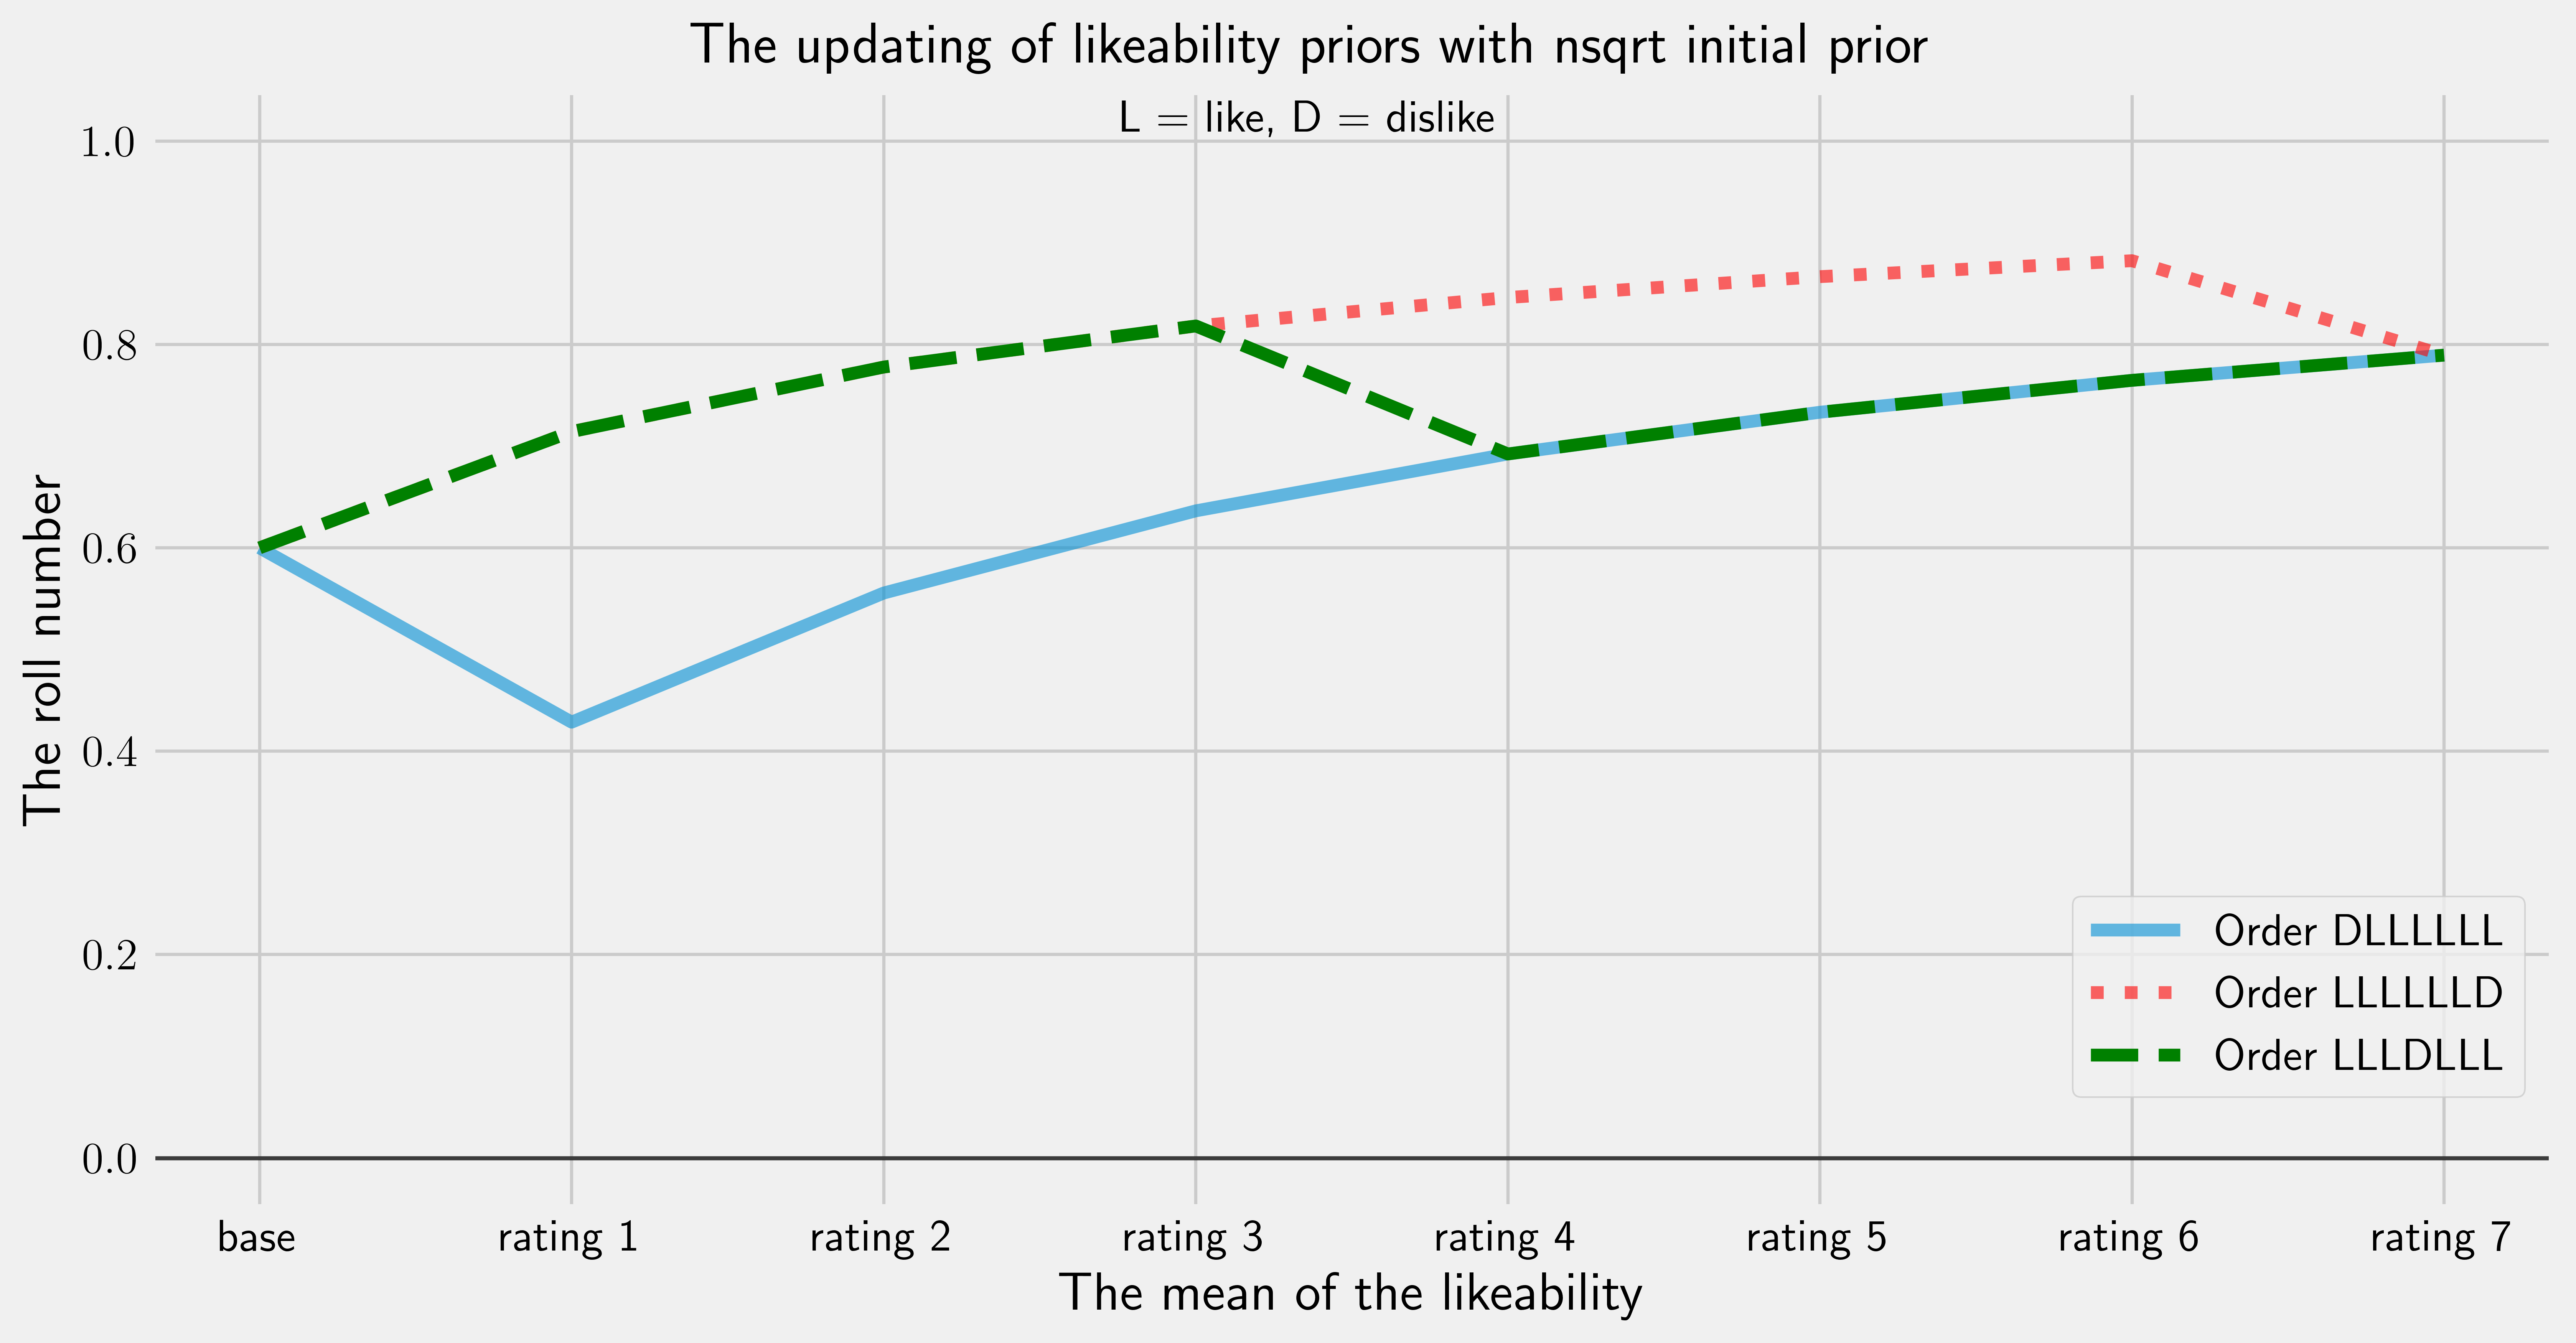
\includegraphics[width=0.9\textwidth]{assets/nsqrt_incre.png}
    \caption{}
    \label{fig:nsqrt_incre}
\end{figure}

% conclude, and table
\subsection{Method Analysis}
At last, the ability to plug in any prior distribution is the main advantage of the Bayesian method, as it will provide a more accurate measurement of likeability for each individual video personally. Furthermore, it provides an accurate metric for comparing between video genres, as I may have different priors and expectations for different types of videos. However, it lacks the neatness of a solution provided by the statistical method and requires a computer to compute the successive priors. Painfully, my algorithm scales in exponential time, making it less applicable as the number of likes and dislikes increase (appendix \ref{apd:algo}). Table \ref{tbl:baye} shows the Bayesian likeability of a nqsrt prior on the five videos.

\begin{figure}[H]
    \centering
    \begin{tabular}{c|c|c|c|c|c}
        & Video A & Video B & Video C & Video D & Video E \\
        \hline
        \hline
        Bayesian Likeability (nsqrt) (3dp) & 0.846 & 0.964 & 0.855 & 0.943 & 0.996
    \end{tabular}
    \captionof{table}{}
    \label{tbl:baye}
\end{figure}

\section{Conclusion}
In this exploration, I investigated a total of five different methods of finding a solution to my problem. Three of the methods have analytic solutions, while two required computers to crunch integrals and random numbers. Due of the variety of the methods, each of them has their pros and cons and usages. While the analytic solutions are the cleanest and easiest to apply with little mental effort, they require the use of algebra manipulations and calculus understandings to derive, and lack the freedom the numerical solution contains. The simulations and the Bayesian method are both computationally intensive, especially at large rating amounts, but does not require much previous knowledge and offers a lot of flexibility in choosing priors, in that order.

Ultimately, I would choose to use the Bayesian likeability with my nsqrt prior as rankings when watching the SoME1 videos. This is because it both accounts for the amount of information available on a video, and fits my prior expectations of the videos. My watching ordering will therefore be: Video E, Video B, Video D, Video C, and Video A. Nevertheless, table \ref{tbl:all}  summaries the likeabilities of the five videos with all methods shown in this exploration.

\begin{figure}[H]
    \centering
    \begin{tabular}{c|c|c|c|c|c}
        & Video A & Video B & Video C & Video D & Video E \\
        \hline
        \hline
         Naive Likeability (3dp) & 1.000 & 1.000 & 0.872 & 1.000 & 0.997\\ \hline
         Simulated Likeability (3dp) & 0.828 & 0.958 &  0.853 & 0.937 & 0.987\\ \hline
         Statistical (Bayesian) Likeability (3dp) & 0.833 & 0.926 & 0.854 & 0.941 & 0.994\\ \hline
        Bayesian Likeability (nsqrt) (3dp) & 0.846 & 0.964 & 0.855 & 0.943 & 0.996
    \end{tabular}
    \captionof{table}{}
    \label{tbl:all}
\end{figure}

This project has been both entertaining to research, and also applicable in a lot of areas that I will be facing in the future for my generalizations. Whether it is finding the best book online given the ratings, or selecting the most favorable bowling place given user reviews, the five methods offer me a spectrum of techniques to statistically analyze the problem. This has been a worthwhile exploration.

% bib
\newpage
%\nocite{*}
\printbibliography


\newpage
\appendix
\counterwithin{figure}{section}
\counterwithin{table}{section}
\section{Figures}

\begin{figure}[H]
    \centering
    \begin{tabular}{c|c|c|c|c|c}
        & 5 likes, 1 dislike & 50, 10 & 500, 100 & 5000, 1000 & 50000, 10000 \\
        \hline
        \hline
        Naive likeability (3dp) & 0.833 & 0.833 & 0.833 & 0.833 & 0.833\\ \hline
        Statistical likeability (3dp) & 0.750 & 0.823 & 0.832 & 0.833 & 0.833\\ \hline
        Difference (3dp) & 0.083 & 0.011 & 0.001 & 0.000 & 0.000
    \end{tabular}
    \captionof{table}{Increase in accuracy of naive method as information size increases}
    \label{apd:acc}
\end{figure}


\begin{figure}[H]
    \begin{pythonln}
import random

def simulate_occurrence(likeability):
    occurrences = 0
    for _ in 0..sample_size:
        likes = 0
        for _ in 0..trials:
            if random() <= likeability:
                likes += 1
            occurrences += likes

    return occurrences
    \end{pythonln}
    % bruh this cant be highlighted using python lmao
    \caption{Implementation of the simulate\_occurrence function with pseudocode}
    \label{apd:sim_occ}
\end{figure}

\begin{figure}[H]
    \begin{pythonln}
from scipy.integrate import quad

def likeability(rolls, prior):
    priors = [...]
    likelihoods = [...]
    evidences = [...]

    priors[0] = prior
    mean = quad(lambda t: t * priors[0](t), 0, 1)

    # exponential time due to recursion
    for index in 0..len(rolls):
        is_like = rolls[index] == 'L'
        if is_like:
            likelihoods[index] = lambda t: t
        else:
            likelihoods[index] = lambda t: 1 - t

        evidences[index] = quad(lambda t: likelihoods[i](t) * priors[i](t),
                               0, 1)
        priors[index+1] = lambda t: likelihoods[i](t) * priors[i](t) \
                                / evidences[i]

        mean = quad(t: t * priors[i+1](t), 0, 1)

    return mean
    \end{pythonln}
    \caption{The algorithm to compute the Bayesian likeability given an initial prior probability density function}
    \label{apd:algo}
\end{figure}

\end{document}
